% ---------------------------------------------------------------------
% --- Arquivo principal e os demais serao os dos capitulos.
% --- EXPRESSÔES ENTRE <> DEVERÂO SER COMPLETADAS COM A INFORMAÇÂO ESPECÌFICA DO TRABALHO 
% ---------------------------------------------------------------------

% Atualizado para atender as normas ABNT por Mônica da Silva (04/11/2021)

%configuração da entrada 
    % 12pt, 	% tamanho da fonte
    %openright, % capítulos começam em pág ímpar (insere página vazia caso preciso)
    % oneside, %% IMPRESSÃO dos elementos textuais e pós-textuais: oneside (apenas no anverso) ou twoside (anverso e verso, se mais de 100 p.) (insere páginas em branco).
    % a4paper, % tamanho do papel. 
    % english, % idioma adicional para hifenização
   	%english,			% idioma adicional para hifenização
	%french,				% idioma adicional para hifenização
	%spanish,			% idioma adicional para hifenização
	%brazil,				% o último idioma é o principal do documento

\documentclass[ruledheader, 12pt, openright, a4paper, oneside, english, brazil]{PPGC_UFF}



%---pacotes para hiphenizacao e acentuacao em portugues
\usepackage[brazil]{babel}
\usepackage[T1]{fontenc}
\usepackage[utf8]{inputenc}	
%\usepackage[latin1]{inputenc}



%--- pacote para figuras
\usepackage{epsf, subfigure}
\usepackage[dvips]{epsfig,graphicx}
\usepackage{chngcntr} %configuração dos padrões numéricos das Figuras e Tabelas
\counterwithout{figure}{chapter} %formata figura para padrão: Figura 1.
\counterwithout{table}{chapter} %formata tabela para padrão: Tabela 1.


%--- pacote de simbolos
\usepackage{pifont,textcomp,latexsym}

%--- simbolos matematicos
\usepackage{amssymb,amstext,amsthm,icomma,amsmath}

%--- pacote para gerar pseudo-codigo
\usepackage{algorithm}
\usepackage{algorithmic}
\floatname{algorithm}{Algoritmo}

%--- outros pacotes
\usepackage{url}
\usepackage{longtable}
\usepackage{lscape}
\usepackage{quoting}

%Tabela Colorida
\usepackage{bigdelim,booktabs, colortbl, longtable, multirow, multicol,rotating }



%%===============================================================================
%% INICIO do Pacotes - Lista de abreviaturas, siglas e acrônimos
%%===============================================================================
		
% Modo "file": utiliza os termos definidos no arquivo acronimos.tex
%  1) Inserção tabular da listas
%  2) Controle da ordem de apresentação das listas
%  3) Não é preciso referenciar no texto
% nonumberlist, %do not show page numbers
% acronym,      %generate acronym listing   -> Not used in this example (see line with)
% toc,          % Inclui a abreviatura no sumário e conta pagina
% section]      %use section level for toc entries
\usepackage[acronym,nopostdot,shortcuts, nonumberlist]{glossaries}


\makeglossaries
\newacronym{DEE}{DEE}{Distância da pele até o espaço epidural}
\newacronym{IMC}{IMC}{Índice de Massa Corporal}
\newacronym{RU}{RU}{Reino Unido}
\newacronym{RV}{RV}{Realidade Virtual}
\newacronym{DoF}{DoF}{degrees of freedom}
\newacronym{ACR}{ACR}{Acronimos}

%%===============================================================================
%% FIM do Pacotes Lista de abreviaturas, siglas e acrônimos
%%===============================================================================

%%===============================================================================
%% Configuração das citações e personalização 
%%===============================================================================

% Os pacotes abaixo só podem ser usados juntamente com o pacote ABNT abaixo e na ordem atual. 
% Esse conjunto de pacotes permite que as citações fiquem na cor azul e sejam usadas como link para as referencias. 
\usepackage[bookmarksopen=true,
            linktoc=page, 
            colorlinks=true,  %ativa a cor do link na referencia
            linkcolor=blue, %muda a cor do link na referencia \ref{} números de tabelas, figuras, seções, sumário etc. 
            citecolor=blue, % muda a cor das citações \cite \textcite
            filecolor=magenta, 
            urlcolor=blue, %muda a cor da url \url no texto e ref. bibliográfica
            ]{hyperref}


\usepackage[ %mais informações de personalização das referencias olhar nos arquivos PDF na pasta MANUAIS OU https://www.overleaf.com/learn/latex/Biblatex_bibliography_styles
    style = abnt, % Sistema alfabético
    %style = abnt-numeric, % Sistema numérico
    %style = abnt-ibid, % Notas de referência
    language=brazil,
    backend=biber,
]{biblatex}

\addbibresource{bibliografia.bib} % A biblioteca para ser utilizada na dissertação/tese.

%%===============================================================================
%% FIM da configuração das citações e personalização 
%%===============================================================================

\hyphenation{
a-de-qua-da-men-te 
di-men-sio-na-men-to 
}

%---------usando tipo de fonte padrão  
% mathptmx (títulos sem negrito) ou ptm (títulos negrito)  - Times - Padrão 
% ugq (títulos negrito) - Arial 
%% --  Padrão do template é: ptm  -- %%
\renewcommand{\ABNTchapterfont}{\bfseries\fontfamily{ptm}\fontseries{b}\selectfont} 
\renewcommand{\ABNTsectionfont}{\bfseries\fontfamily{ptm}}


% --- -----------------------------------------------------------------
% --- Documento Principal.
% --- -----------------------------------------------------------------

\begin{document}


% --- -----------------------------------------------------------------
% --- Titulo, abstract, dedicatórias e agradecimentos.
% --- Índice geral, lista de figuras e tabelas.
% --- -----------------------------------------------------------------
% Atualizado para atender as normas ABNT por Mônica da Silva (04/11/2021)

% --- -----------------------------------------------------------------
% --- Elementos usados na Capa e na Folha de Rosto.
% --- EXPRESSÔES ENTRE <> DEVERÂO SER COMPLETADAS COM A INFORMAÇÂO ESPECÍFICA DO TRABALHO
% --- E OS SÌMBOLOS <> DEVEM SER RETIRADOS 
% --- -----------------------------------------------------------------
\autor{RAFAEL HEITOR CORREIA DE MELO} % deve ser escrito em maiúsculo

\titulo{Uma Proposta de Uso de Dispositivo Háptico
para Treinamento de Anestesia Raquidiana}

\instituicao{UNIVERSIDADE FEDERAL FLUMINENSE}

\orientador{Aura Conci, D.Sc.}

%\coorientador{<NOME DO COORIENTADOR>} % se nao existir co-orientador apague essa linha

\local{NITER\'{O}I}

\data{2022} % ano da defesa

\comentario{Tese de Doutorado apresentada ao Programa de P\'{o}s-Gradua\c{c}\~{a}o em Computa\c{c}\~{a}o da \mbox{Universidade} Federal Fluminense como requisito parcial para a obten\c{c}\~{a}o do Grau de \mbox{Doutor em Computa\c{c}\~{a}o}. \'{A}rea de concentra\c{c}\~{a}o: \mbox{Computação Visual.}} %preencha com a sua área de concentração


% --- -----------------------------------------------------------------
% --- Capa. (Capa externa, aquela com as letrinhas douradas)(Obrigatório)
% --- ----------------------------------------------------------------
\capa

% --- -----------------------------------------------------------------
% --- Folha de rosto. (Obrigatório)
% --- ----------------------------------------------------------------
\folhaderosto

% --- -----------------------------------------------------------------
% --- Ficha catalográfica obrigatória na versão final. (Obrigatório)
% --- ----------------------------------------------------------------

\begin{figure}[!ht]
   \centering
   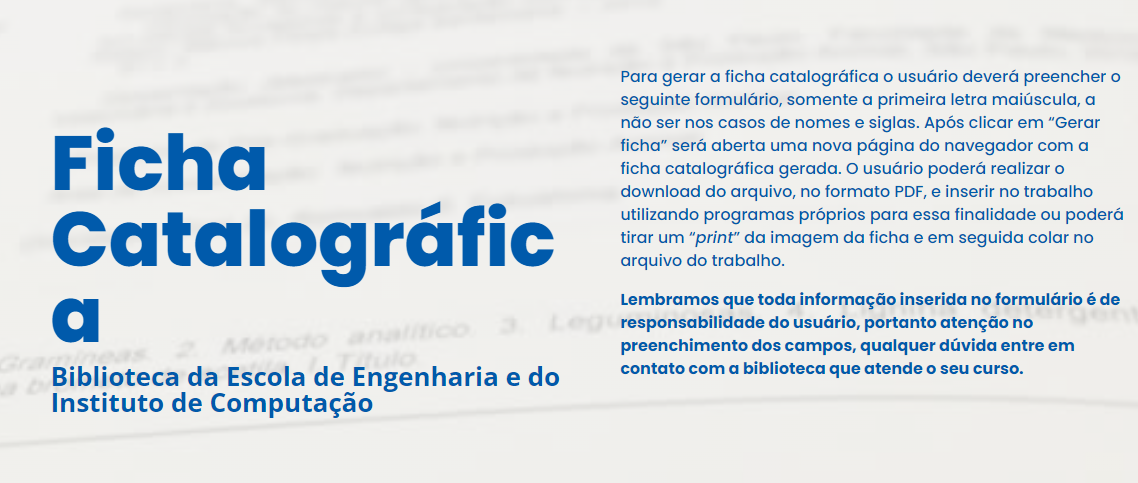
\includegraphics[width=1\linewidth]{capitulos/figuras/ficha_catalografica.png}
   \caption{Local da ficha catalográfica}
\end{figure}

\cleardoublepage


\pagestyle{ruledheader}
\setcounter{page}{1}
\pagenumbering{roman}

% --- -----------------------------------------------------------------
% --- Termo de aprovação. (Obrigatório)
% --- ----------------------------------------------------------------
\cleardoublepage
\thispagestyle{empty}

\vspace{-60mm}

\begin{center}
   {\large RAFAEL HEITOR CORREIA DE MELO}\\
   \vspace{7mm}

   Uma Proposta de Uso de Dispositivo Háptico
para Treinamento de Anestesia Raquidiana\\
  \vspace{10mm}
\end{center}

\noindent
\begin{flushright}
\begin{minipage}[t]{8cm}

Tese de Doutorado apresentada ao Programa de P\'{o}s-Gradua\c{c}\~{a}o em Computa\c{c}\~{a}o da Universidade Federal Fluminense como requisito parcial para a obten\c{c}\~{a}o do \mbox{Grau} de Doutor em Computa\c{c}\~{a}o. \'{A}rea de concentra\c{c}\~{a}o: \mbox{Ciência da Computação.} %preencha com a sua área de concentração

\end{minipage}
\end{flushright}
\vspace{1.0 cm}
\noindent
Aprovada em outubro de 2022. \\
\begin{flushright}
 % \parbox{11cm}
  {
  \begin{center}
  BANCA EXAMINADORA \\
  \vspace{6mm}
  \rule{11cm}{.1mm} \\
    Profa. D.Sc. Aura Conci - Orientadora, UFF \\
    \vspace{6mm}
  \rule{11cm}{.1mm} \\
    Prof. D.Sc. Anselmo Cardoso de Paiva, UFMA\\
    \vspace{6mm}
  \rule{11cm}{.1mm} \\
    Prof. D.Sc. Débora Christina Muchaluat Saade, UFF\\
  \vspace{4mm}
  \rule{11cm}{.1mm} \\
    Prof. D.Sc. Fátima de Lourdes dos Santos Nunes Marques, USP\\
    \vspace{6mm}
  \rule{11cm}{.1mm} \\
    Prof. D.Sc. José Viterbo Filho, UFF\\
  \vspace{6mm}
  \end{center}
  }
\end{flushright}
\begin{center}
  \vspace{4mm}
  Niter\'{o}i \\
  %\vspace{6mm}
  2022

\end{center}

% --- -----------------------------------------------------------------
% --- Dedicatoria.(Opcional)
% --- -----------------------------------------------------------------
\cleardoublepage
\thispagestyle{empty}
\vspace*{200mm}

\begin{flushright}
{\em 
    %Dedicatória(s): Elemento opcional onde o autor presta homenagem ou dedica seu trabalho (ABNT, 2005).
    
    Dedico este trabalho a minha esposa, Evelyn, que sempre me apoiou na direção das minhas conquistas e ao meu filho, Rafael, que, ao chegar me apresentou uma nova forma de amar.
}
\end{flushright}
\newpage


% --- -----------------------------------------------------------------
% --- Agradecimentos.(Opcional)
% --- -----------------------------------------------------------------
\pretextualchapter{Agradecimentos}
\hspace{5mm}
%<Elemento opcional, colocado após a dedicatória (ABNT, 2005). >
Agradeço a Deus por me mostrar sempre os caminhos, mesmo nos momentos em que parece que isso não vai acontecer. 

Aos meus pais Julio e Dayse pela preocupação e apoio. Aos meus irmãos Leonardo e Julia pela amizade e companheirismo essenciais nos momentos difíceis.

Agradeço muito a minha orientadora Aura, que mesmo nos momentos de desânimo conseguiu me trazer, em palavras, motivação para seguir em frente.

Ao amigo André que foi essencial em parte dessa caminhada.

À minha família, agradeço a compreensão pelas minhas ausências e minhas desculpas nos momentos de desânimo.



% --- -----------------------------------------------------------------
% --- Resumo em português.(Obrigatório)
% --- -----------------------------------------------------------------
\begin{resumo}

%Elemento obrigatório, constituído de uma sequência de frases concisas e objetivas e não de uma simples enumeração de tópicos, não ultrapassando 500 palavras ABNT NBR 6028:2003.

As anestesias raquidianas são procedimentos cegos que dependem do sentimento do médico no decorrer da inserção da agulha para correta identificação do local de aplicação do líquido anestésico. Em grande parte dos centros de treinamento a primeira experiência tátil do médico em treino tende a ser praticada em pacientes reais. Esta prática, apesar de ser efetuada sob supervisão direta, traz riscos para estes pacientes e inseguranças aos aprendizes. Técnicas alternativas de uso de \textit{phantoms} e cadáveres no treinamento oferecem uma pequena representatividade em relação às variações de pacientes reais. 
Nesta tese desenvolvemos um ambiente virtual para simulação do procedimento que envolve anestesias raquidianas. Considera-se o procedimento de punção com \textit{feedback} tátil e visual usando técnicas de autotreinamento. As sensações táteis do médico em treinamento são simuladas no protótipo através da integração com dispositivo háptico. A geração e visualização dinâmica de modelos de corpos de pacientes baseados em altura e peso foi desenvolvida a partir de uma criteriosa revisão bibliográfica de trabalhos anteriores sendo uma parte muito importante deste trabalho. Alunos de computação validaram a parte do protótipo que envolve a detecção de diferentes sensações de perfuração de tecidos por meio de experimentos propostos. Ainda foi criado e usado aqui um modelo adaptável de um corpo de gestante que possui modelagem de todas as camadas desde a pele das costas até os ossos da coluna vertebral. Modelamos de forma dinâmica as camadas de tecido mais variáveis para permitir uma maior variabilidade de cenários de treinamento. Finalmente, incluímos também uma variação das etapas de treinamento de acordo com a detecção automática do nível de habilidade da pessoa na execução de cada procedimento. Pessoas com execução insatisfatória terão que executar mais procedimentos durante o seu treinamento. Os erros são reportados durante cada procedimento para possibilitar a evolução na prática do aprendiz.

{\hspace{-8mm} \bf{Palavras-chave}}: Dispositivo háptico, Treinamento médico, Anestesia raquidiana, Realidade virtual, Ambiente virtual, Paciente virtual Simulação, Retorno tátil.

\end{resumo}

% --- -----------------------------------------------------------------
% --- Resumo em língua estrangeira.(Obrigatório)
% --- -----------------------------------------------------------------
\begin{abstract}

%Elemento obrigatório, em língua estrangeira, com as mesmas características do resumo em língua vernácula (ABNT, 2005).

Spinal anesthesia is a blind procedure where physicians rely on manual feedback to guide their movements through needle insertion. The aim is to identify drug administration locations correctly. For many training centers, the first tactile experience of anesthetists in training occurs in an actual patient under direct supervision. Besides this supervision, there are risks associated with this approach for patients and apprentices. Using phantoms and dead bodies for training offers a low range of scenarios. In this thesis, we developed a virtual environment for simulating the procedure that involves spinal anesthesia. The puncture procedure is considered with tactile and visual feedback using self-training techniques. The tactile sensations of the physician in training are simulated in the prototype through integration with a haptic device. The dynamic generation and visualization of models of patients' bodies based on height and weight was developed from a careful bibliographic review and is a significant part of this work. Computer science students validated the detection of different sensations of tissue perforation related to the procedure through experiments. An adaptable model of a pregnant woman's body was created and used here. We include in the model all layers from the skin of the back to the spine's bones. To allow more significant variability of training scenarios, we included the dynamic possibility of growth to most variable tissue layers. Finally, we also included a variation of the training steps according to the automatic detection of the person's skill level in performing each procedure. People with poor execution will have to perform more procedures during their training. Errors are reported during each procedure to allow progress in the learner's practice. 



% O resumo deve ser redigido na terceira pessoa do singular, com verbo na voz ativa, não ultrapassando uma página ou 500 palavras, segundo a ABNT NBR 6028). Evitando-se ouso de parágrafos no meio do resumo, assim como fórmulas, equações e símbolos. Iniciar o resumo situando o trabalho no contexto geral, apresentar os objetivos, descrever a metodologia utilizada, relatar a contribuição própria, comentar os resultados obtidos e finalmente apresentaras conclusões mais importantes do trabalho. 



{\hspace{-8mm} \bf{Keywords}}: Haptics, Medical training, Spinal anesthesia, Virtual reality, Virtual environment, Virtual patient, Simulation, tactile feedback.

\end{abstract}

% --- -----------------------------------------------------------------
% --- Lista de figuras.(Opcional)
% --- -----------------------------------------------------------------
%\cleardoublepage
\listoffigures



% --- -----------------------------------------------------------------
% --- Lista de tabelas.(Opcional)
% --- -----------------------------------------------------------------
\cleardoublepage
%\label{pag:last_page_introduction}
\listoftables
\cleardoublepage

% --- -----------------------------------------------------------------
% --- Lista de abreviatura.(Opcional)
%Elemento opcional, que consiste na relação alfabética das abreviaturas e siglas utilizadas no texto, seguidas das %palavras ou expressões correspondentes grafadas por extenso. Recomenda-se a elaboração de lista própria para cada %tipo (ABNT, 2005).
% --- ----------------------------------------------------------------

\cleardoublepage
\printglossary[type=\acronymtype,title={Lista de Abreviaturas e Siglas}]
\cleardoublepage


% --- -----------------------------------------------------------------
% --- Sumario.(Obrigatório)
% --- -----------------------------------------------------------------

\pagestyle{ruledheader}
\tableofcontents
\pagebreak %na pasta capítulos

% --- -----------------------------------------------------------------
% --- Inserção dos capítulos.
% --- todos os arquivos estão na pasta capítulos
% --- -----------------------------------------------------------------

\setcounter{page}{1} %parâmetros da contagem de paginas.
\pagenumbering{arabic} %padrão de números de paginas em arábico (1,2,3) 
\setcounter{page}{12} %inicia a contagem das paginas 12 - folha de rosto e considera a pagina da 

\pagestyle{ruledheader}

%%%% CAPÍTULO 1 - INTRODUÇÃO
%%
%% Deve apresentar uma visão global da pesquisa, 
%% incluindo: breve histórico, importância e
%% justificativa da escolha do tema, delimitações
%% do assunto, formulação de hipóteses e objetivos
%% da pesquisa e estrutura do trabalho.

% Perguntas que podem guiar a introdução - não necessariamente irá ter a resposta para tudo, isso depende da área.
% 1 - Qual é o contexto em que seu trabalho está inserido?
% 2 - Qual é o problema que motiva a existência deste trabalho?
% 3 - Qual é a visão geral da literatura sobre o problema e como é tratado
% 4 - Por que a solução na literatura não é o suficiente para ?
% 5 - Como seu trabalho trata o problema ?
% 6 - como seu trabalho foi avaliado para comprovar que tratou adequadamente o problema?
% 7 - De forma geral quais foram os resultados ?
% 8 - Quais foram as contribuições do seu trabalho?
% 9 -  Como o restante da Dissertação ou Tese está organizada ?


\chapter{Introdução}
\label{cap:introducao}

Nas anestesias raquidianas os anestesistas dependem da sua sensação tátil durante a inserção da agulha no paciente para a correta identificação do local de aplicação do líquido anestésico. O local de aplicação da raquidiana é conhecido como espaço subaracnóideo \cite{Miller2009}). Para que o anestesista reconheça a chegada da agulha neste local ele precisa reconhecer os tecidos perfurados no caminho dela. As anestesias possuem técnicas específicas para identificação dos seus espaços de aplicação. Para que os médicos dominem a técnica da anestesia raquidiana é estimado que são necessários 44 ± 6 repetições de execução deste tipo de procedimento \cite{Kopacz1996}. A confirmação de que o local adequado foi atingido na anestesia raquidiana é feita através da observação do vazamento, por meio da agulha de punção, do liquido cérebro espinhal ou cefalorraquidiano (\textit{líquor}). As Figuras~\ref{fig:puncaoLombar} e~\ref{fig:gotejamentoLiquor} ilustram dois momentos importantes da anestesia raquidiana retirados do vídeo de \textcite{Londero2018} disponível no link\footnote{\url{https://www.youtube.com/watch?v=Dl8ijvHVTuY&ab_channel=CLAUDINEILONDERO}}. Na Figura~\ref{fig:puncaoLombar} é mostrado o momento de inserção da agulha para punção lombar e na Figura~\ref{fig:gotejamentoLiquor} é mostrado o vazamento, através da agulha de punção, do \textit{líquor}, o que acontece alguns segundos após a agulha estar corretamente posicionada no espaço subaracnóideo. Neste tipo de anestesia é usada uma agulha de menor diâmetro do que a agulha utilizada na anestesia epidural \cite{Miller2009}. O ultrassom é uma ferramenta eficiente para auxílio na determinação do espaço onde a agulha precisa ser inserida \cite{Helayel2010, Soni2019} bem como na definição da espessura das diversas camadas de tecido \cite{Klingensmith2022}. Existem inclusive soluções desenvolvidas para interpretação de imagens de ultrassom que vem sendo estudadas para substituir a apalpação do anestesista na determinação do ponto de inserção da agulha \cite{Ni2021}. Porém, o uso de equipamentos de ultrassom para este fim não é uma realidade em muitos centros no Brasil \cite{Hamaji2016}. O uso deste equipamento ou qualquer outra técnica \cite{Berde2022}, portanto não faz parte do treinamento de muitas faculdades de medicina para anestesias raquidianas. A determinação do ponto de inserção da agulha no treinamento, assim como no procedimento real em pacientes, é comumente feita fazendo uso de referências anatômicas através da apalpação da crista ilíaca do paciente. A crista ilíaca pode ser observada nas imagens da Figura~\ref{fig:cristaIliaca} \cite{Moura2019}. 

\begin{figure}[!ht]
   \centering
   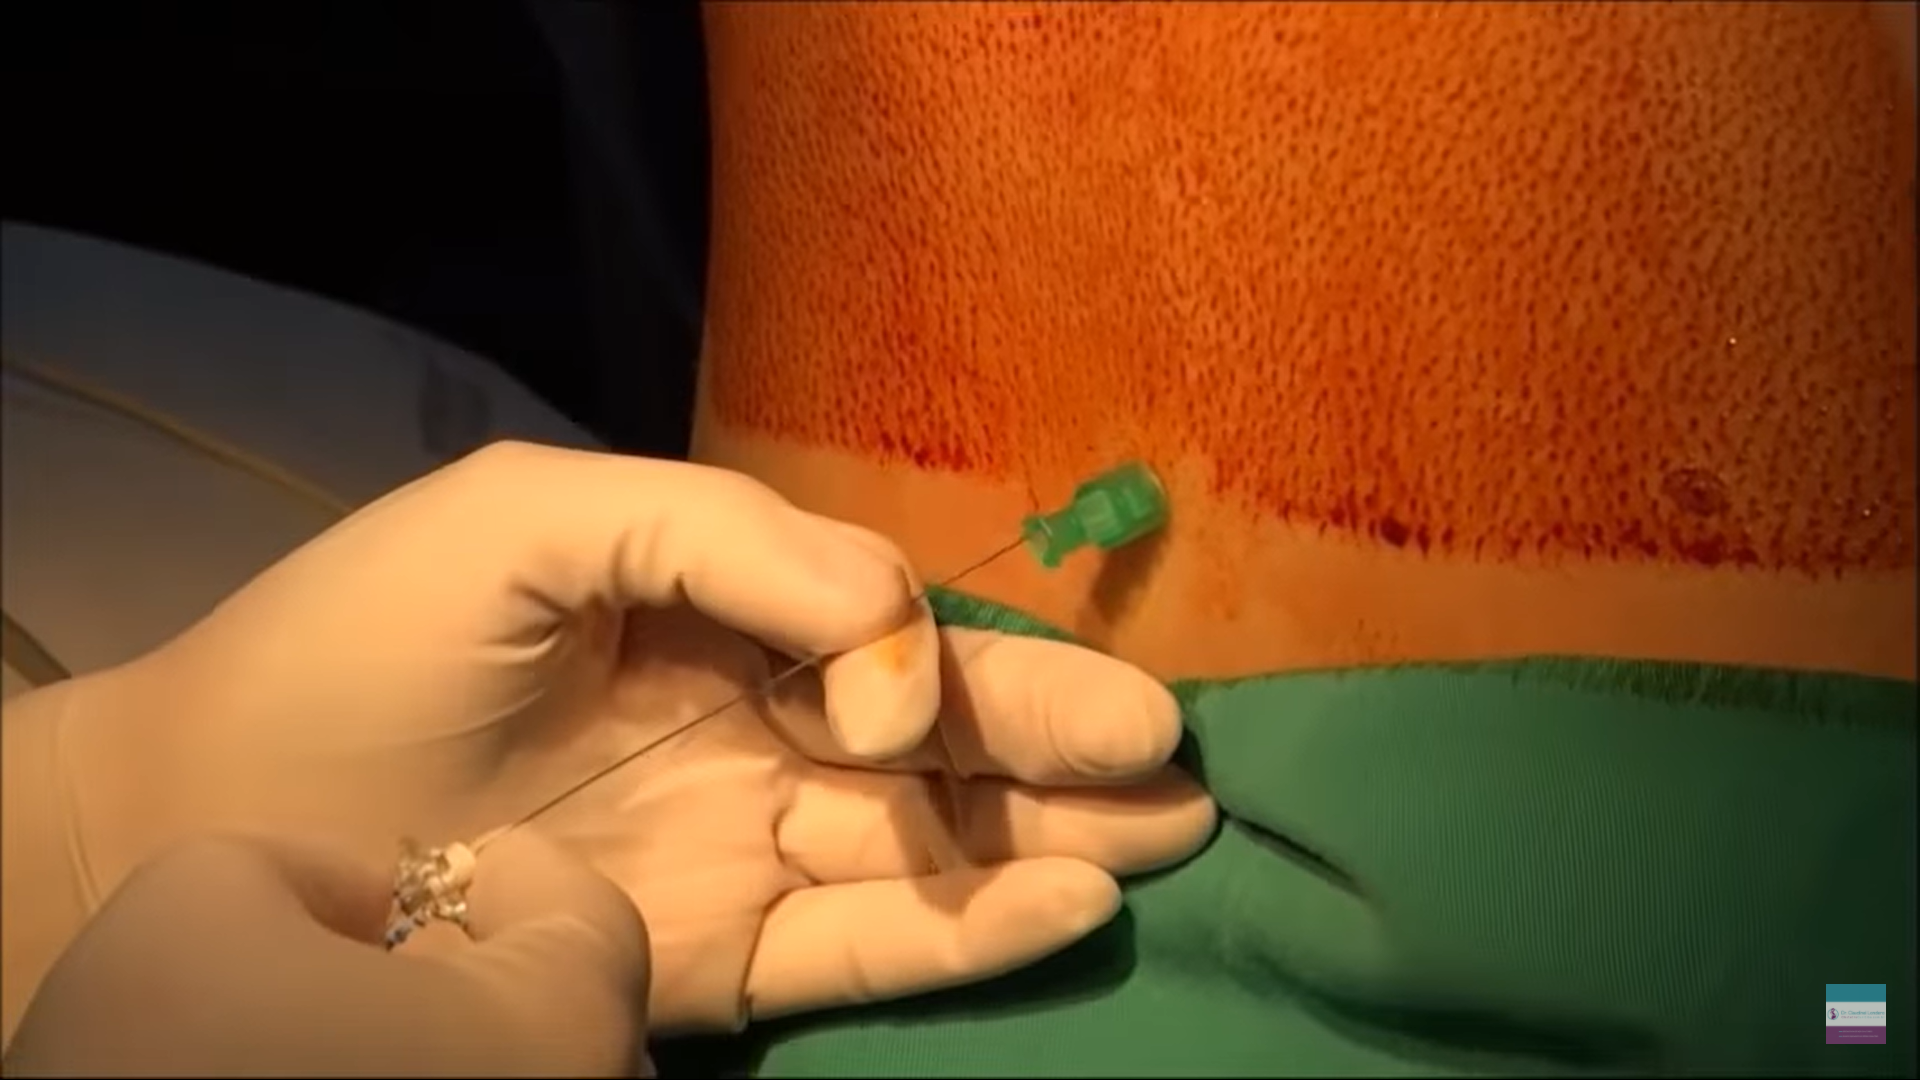
\includegraphics[width=0.6\linewidth]{capitulos/figuras/2.PuncaoLombar.png}
   \caption{Punção lombar com agulha de raquianestesia  \cite{Londero2018}.}
   \label{fig:puncaoLombar}
\end{figure}

\begin{figure}[!ht]
   \centering
   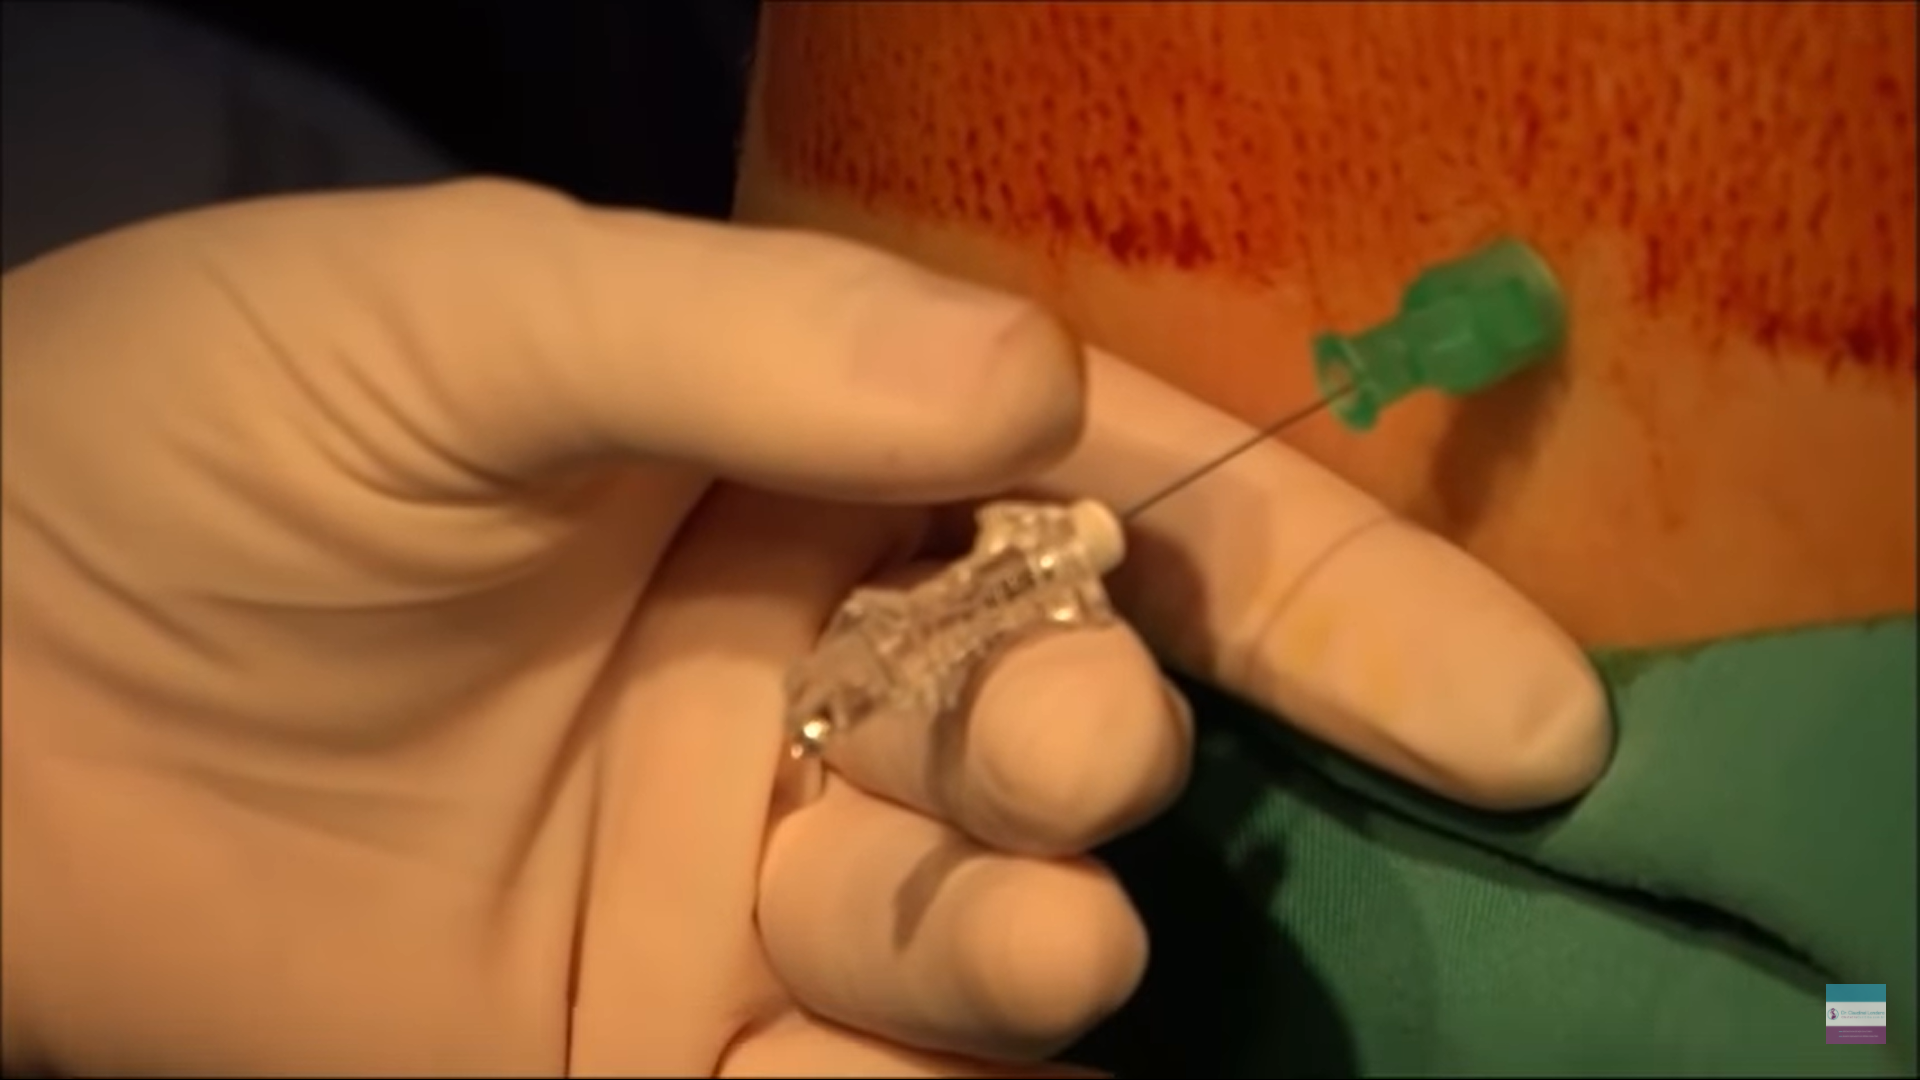
\includegraphics[width=0.6\linewidth]{capitulos/figuras/3.GotejamentoLiquor.png}
   \caption{Gotejamento do \textit{líquor}, indicação do local correto para a raquianestesia \cite{Londero2018}.}
   \label{fig:gotejamentoLiquor}
\end{figure}

\begin{figure}[ht!]
    \centering
        \begin{tabular}{cc}
        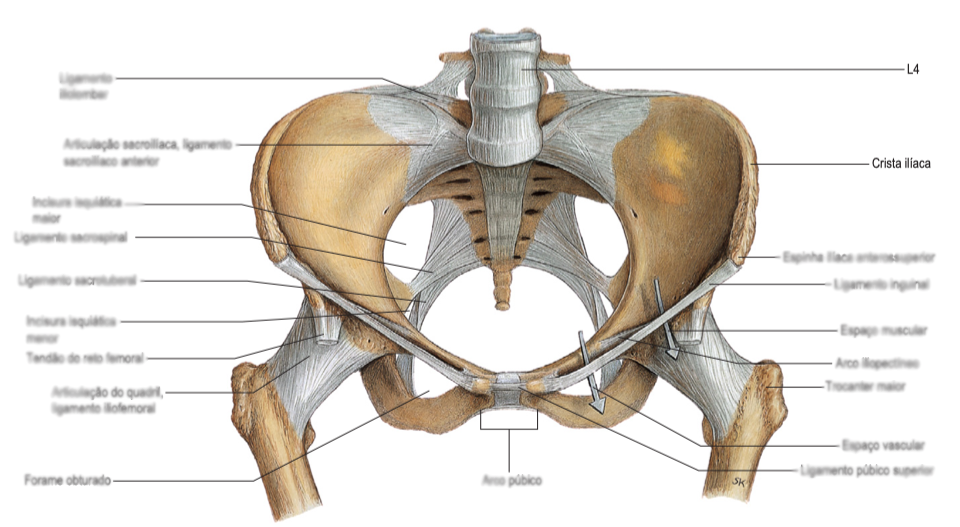
\includegraphics[width=0.55\linewidth]{capitulos/figuras/crista-iliaca-pelve-ossos-ligamentos.png} & 
        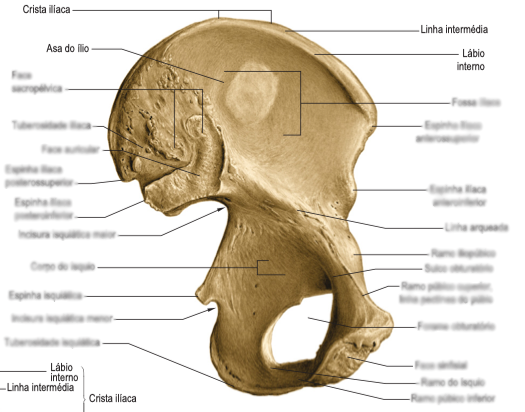
\includegraphics[width=0.35\linewidth]{capitulos/figuras/crista-iliaca-ossos-quadril.png} 
        \\
        (a) & (b)
        \end{tabular}
    \caption{Ilustração da crista ilíaca através de duas imagens dos ossos da pelve \cite{Moura2019}. Nas imagens a indicação de elementos que não estão diretamente relacionados à crista ilíaca foram embaçados de forma a simplificar a visualização desta: (a) Vista frontal (b) Vista lateral.}
    \label{fig:cristaIliaca}
\end{figure}

A principal abordagem de treinamento para técnicas de anestesia envolve a observação da aplicação das técnicas por anestesistas experientes \cite{Vrillon2022}. Estes orientam verbalmente os aprendizes conforme cada um dos passos é executado. Adicionalmente a isto são usados: desenhos 2D, cadáveres para demonstração do procedimento, apresentação de vídeos das técnicas sendo executadas em pacientes, visualização 3D \cite{Vrillon2022} e técnicas de simulação. No que diz respeito ao treinamento das sensações táteis além do uso de cadáveres alguns simuladores fazem uso de bonecos com tecidos artificiais, denominados \textit{phantoms}, que simulam pacientes \cite{Dreifaldt2006, KyotoKagaku2015, Mashari2018}. Um ponto negativo importante no uso de \textit{phantoms} e de cadáveres, talvez o principal, é a baixa representatividade no que diz respeito a reprodução da situação real, pois estes oferecem uma baixa variabilidade de cenários (variações possíveis dos corpos dos pacientes) para treinamento. Esta fato fica notório na análise destes tipos de simuladores feita na Seção \ref{sec:SimuladoresPhantoms}. A maior quantidade de tipos de corpos representado pelos \textit{phantoms} nos simuladores estudados foi de 4 enquanto é sabido que a variabilidade das estruturas corporais mesmo em uma população pequena é muito maior do que isso. Outro aspecto relevante no uso de \textit{phantoms} é a necessidade de reposição de peças que se desgastam com o uso e podem ter custos altos. Estes são alguns dos motivos para que em diversos hospitais a primeira experiência do anestesista em treinamento seja efetuada diretamente em um paciente \cite{Aggarwal2009, Grantcharov2008, Smith2005, Watterson2007}. Esta prática, apesar de ser efetuada sob supervisão direta de médicos experientes, pode trazer riscos para as pessoas que são anestesiadas (pacientes) e uma maior propensão a inseguranças por parte dos aprendizes \cite{Elmofty2017}. 

O uso de simuladores para adquirir certo grau de habilidade antes de iniciar o procedimento em pacientes minimiza os riscos tanto para o aprendiz quanto para o paciente não só na anestesia \cite{Escobar-Castillejos2016, Yunoki2018} como em diversas outras áreas da medicina \cite{Akhtar2014, Alvarez-Lopez2020, Hamm2022}. A existência de diversos cenários em simuladores como os que usam \acrfull{RV} auxilia e motiva o ensino e possibilita ao aprendiz ter experiência com situações mais variadas assim como aumenta a segurança dos alunos. Essa técnica tem também a vantagem de possibilitar que a avaliação do desempenho destes seja feita de forma automatizada e padronizada \cite{Willis2014}. 

Estes simuladores com frequência usam diferentes níveis variando as dificuldades \cite{Ullrich2012}. Possibilitam a redução ou eliminação de custos de manutenção de equipamentos e laboratórios físicos bem como evitam a necessidade de estruturação de laboratórios \cite{Silva2018}. 
Esta variabilidade de cenários dificilmente aconteceria na vida real em centros onde o ensino é feito diretamente em pacientes \cite{Udani2015}. No cenário de treinamento diretamente em pacientes a experiência inicial de cada anestesista pode ser muito distinta uma vez que estas dependem da estrutura corporal do paciente atendida por cada residente. Esta não é uma abordagem ideal para treinamentos uma vez que cria uma dependência no que diz respeito à experiência tátil dos anestesistas novatos em uma variável que não está sob o controle do profissional responsável pelo treinamento. Cada aluno pode vir a ter uma gama diferente de experiências a depender das características físicas dos pacientes que este teve suas primeiras experiências. Isto impacta o nivelamento do ensino.

Diversos simuladores utilizam dispositivos de força háptica (\textit{force feedback}) para auxiliar o aprendiz a experimentar fisicamente as sensações de resistência modeladas para os tecidos ao praticar procedimentos médicos. Este tipo de abordagem é usada em procedimentos médicos de um modo geral \cite{Escobar-Castillejos2016, Patel2021} assim como no caso mais específico dos procedimentos de anestesia \cite{Vaughan2013, Collaco2021}. Existem muitas outras formas de como o uso de ferramentas computacionais pode auxiliar no campo da anestesia. Um exemplo é no controle automatizado de quanto anestésico aplicar a partir de respostas de medições dos níveis de consciência do paciente \cite{Mendez2009}. Outro exemplo é uso da imersão \acrshort{RV} durante a cirurgia em conjunto com a anestesia como forma de reduzir a dor e estimular o relaxamento diminuindo a ansiedade e possivelmente a quantidade de anestésico necessário \cite{Eijlers2019}.

\textcite{Correa2019}, na sua análise do estado da arte, relataram que as avaliações da percepção humana são pouco exploradas no campo da interação háptica para treinamento de inserção de agulhas. Eles também citam a predominância de testes subjetivos para validação das soluções propostas por parte dos usuários. Alguns trabalhos fazem uso de análises subjetivas usando gráfico de profundidade da agulha versus tempo como em \textcite{Magill2010}. 

O trabalho desta tese foi iniciado com a apresentação do simulador de \textcite{Brazil2017thesis} para um anestesista com o intuito de agregar a este simulador outro tipo de anestesia, no caso a anestesia raquidiana. A proposta inicial desta tese propunha a utilização destes simuladores para a avaliação de ganho de conhecimento no treinamento de novos anestesistas com o uso do simuladores em comparação com a ausência do seu uso. A opinião do especialista foi a de que este tipo de avaliação seria mensurável de forma mais concreta para o simulador de raquianestesia. A partir de estudos do estado da arte foi observado que os simuladores que possibilitam a anestesia raquidiana não contemplam algumas das principais características desejáveis para a correta representação do procedimento como por exemplo a apalpação da coluna para determinação do ponto de inserção da agulha. Com isto um simulador de anestesia raquidiana foi construído visando atender as principais demandas do treinamento das sensações envolvidas neste procedimento. Na literatura estudada foram adotadas diversas formas de abordar o problema do treinamento de anestesias regionais. Simuladores deste tipo possuem muitas características relevantes o que faz com que o foco no atendimento em algumas geralmente venha a comprometer outras. Grande parte dos simuladores computacionais de anestesia estudados apresenta como opção para o usuário somente a simulação de anestesias epidurais e não de raquianestesias que é o foco desta tese.

A apresentação de cenários de treinamento virtuais que simulam a possibilidade de visualização e sentimentos táteis que são vivenciados no procedimento real visa aproximar a prática de treino virtual da posterior prática em pacientes reais. Desta forma, possibilita um maior sentimento de segurança por parte dos anestesistas aprendizes. A aplicação de transparência em camadas foi uma das técnicas que foi incluída no ambiente virtual de treinamento criado nesta tese. Esta funcionalidade permite a visão do interior do corpo o que facilita o entendimento do aprendiz no que diz respeito à teoria do procedimento. Esta conexão da teoria com a prática é um grande trunfo no uso da \acrfull{RV} em simuladores para treinamento. Neste caso, o realismo na apresentação dos elementos envolvidos no treinamento tem um papel importante. Seja a representação 3D da agulha, do corpo ou das camadas internas que possam ser visualizadas. 

\section{Definição do problema}
\newtheorem{prob}{Problema}

Esta tese de doutorado define a seguinte questão de pesquisa a ser estudada e solucionada por este trabalho.

\begin{prob}
\label{prob:simuladorCasoReal}
    É possível criar uma ferramenta virtual para treinamento médico que auxilie no treinamento do procedimento de raquianestesia a partir do uso de realidade virtual e com dispositivo háptico de forma a simular este procedimento desde a palpação da coluna (para determinação do ponto de inserção da agulha)?
\end{prob}

Dentre os simuladores de raquianestesia computacionais atuais não existe um que contemple na simulação a palpação do corpo pelo médico anestesista para determinação do ponto de inserção da agulha. Esta opção existe para somente dois simuladores de anestesia epidurais estudados nesta tese sendo que somente em um deles este procedimento é feito de maneira 100\% virtual como propomos neste trabalho. O simulador epidural que possibilita simulação de apalpação não teve a sua solução avaliada por especialistas. 

\section{Objetivos}
\label{sec:objetivos}

Esta tese tem o seguinte objetivo geral:

Propor e desenvolver um ambiente de treinamento virtual no que se refere às técnicas de anestesia raquidiana em gestantes desde a apalpação para determinação do ponto de inserção da agulha até a administração do anestésico no local correto. A ideia é prover um aprendizado prático, didático e mais completo dos anestesistas sem incorrer em risco para os pacientes e estresse para os anestesistas em treinamento. Este treinamento será padronizado no sentido das técnicas que precisarão ser dominadas pelos usuários treinados. O sistema irá fazer com que os usuários que demonstrarem melhor desenvoltura nas etapas iniciais evoluam mais rapidamente pelas etapas de demonstração de habilidades já entendidas e aprendidas. 

Dentre os objetivos específicos pode-se destacar:
\begin{enumerate}
\item Possibilitar variações das situações possíveis de ocorrer em relação às características físicas das pacientes; 
\item Desenvolver modelagens que mapeiam as características físicas na visualização; 
\item Possibilitar visualização dos tecidos internos no momento da anestesia para auxílio no aprendizado inicial. 
\item Utilizar técnicas de realidade virtual na representação da paciente e dos equipamentos usados no procedimento em ambiente 3D interativo;
\item Empregar dispositivos hápticos como meio de interação para simular os sentimentos táteis do médico (de forma semelhante ao procedimento real em treinamento);
\item Dar retorno ao usuário em relação as ações feitas corretas e incorretas no que diz respeito ao procedimento visando auxiliar na evolução do seu desempenho.
\end{enumerate}

\section{Contribuições da Tese}
\label{sec:contribuicoes}

Uma das principais contribuições deste trabalho envolve a reprodução virtual das principais sensações hápticas necessárias para simular a anestesia raquidiana. Outra contribuição foi a construção de um modelo 3D real da parte lombar do corpo de uma gestante (tecidos entre a pele e a cauda equina) de forma facilmente modificável via programação. A variação dos tamanhos das principais camadas do modelo foi alimentada por um equação genérica criada e detalhada neste trabalho. Foi criado então um ambiente para treinamento de raquianestesia que apresenta \textit{feedbacks} durante e após cada
procedimento bem como uma proposta de avaliação de desempenho por meio de notas.

\section{Estrutura da Tese}
\label{sec:estrutura}

O restante do texto está estruturado da seguinte forma. O Capítulo~\ref{cap:cap2} comenta os principais conceitos e tecnologias envolvidas no desenvolvimento do ambiente de treinamento proposto.

O Capítulo~\ref{cap:cap3} contém os trabalhos relacionados a esta tese assim como o posicionamento deste trabalho frente aos demais.

No Capítulo~\ref{cap:cap4} é apresentada a especificação do ambiente de treinamento que foi desenvolvido durante esta tese. 

A implementação do ambiente de treinamento que foi desenvolvido durante esta tese está descrita no Capítulo~\ref{cap:cap5}. 

O Capítulo~\ref{cap:cap6} apresenta os experimentos que foram feitos e uma avaliação destes em relação aos seus resultados.

Por fim, o Capítulo~\ref{cap:cap7} conclui o trabalho, apresentando as conclusões, realçando as contribuições desta tese e apontando as limitações e os  trabalhos futuros.




%\pagestyle{ruledheader}
%\chapter{Fundamentação Teórica} \label{cap:cap2}

Este Capítulo relaciona os conceitos e as tecnologias envolvidas no desenvolvimento do ambiente de treinamento proposto. 

\section{Anestesias Regionais}

Anestesias são atualmente usadas em diversos procedimentos cirúrgicos na medicina tradicional com o intuito de bloquear temporariamente a capacidade do cérebro de reconhecer um estímulo doloroso. Esta prática visa permitir a execução de procedimentos invasivos por parte do médico enquanto mantém o conforto e a tranquilidade do paciente. A anestesia regional é um procedimento usado em cirurgias onde o paciente pode permanecer acordado. Este tipo de anestesia bloqueia a dor em apenas uma determinada região do corpo, como um braço, uma perna ou toda região inferior do corpo, abaixo do abdômen \cite{Pinheiro2018}.

Os dois tipos de anestesias regionais mais usados são: anestesia raquidiana (ou raquianestesia, raqui), e anestesia peridural ou epidural. Estes dois tipos de anestesias também são conhecidas como anestesias de neuroeixo ou ainda bloqueio de neuroeixo \cite{Pinheiro2018}. Ambas podem ser aplicadas com pacientes sentados e inclinados para frente ou deitados de lado \cite{Anesclin2019}. 

\begin{figure}[ht!]
    \centering
    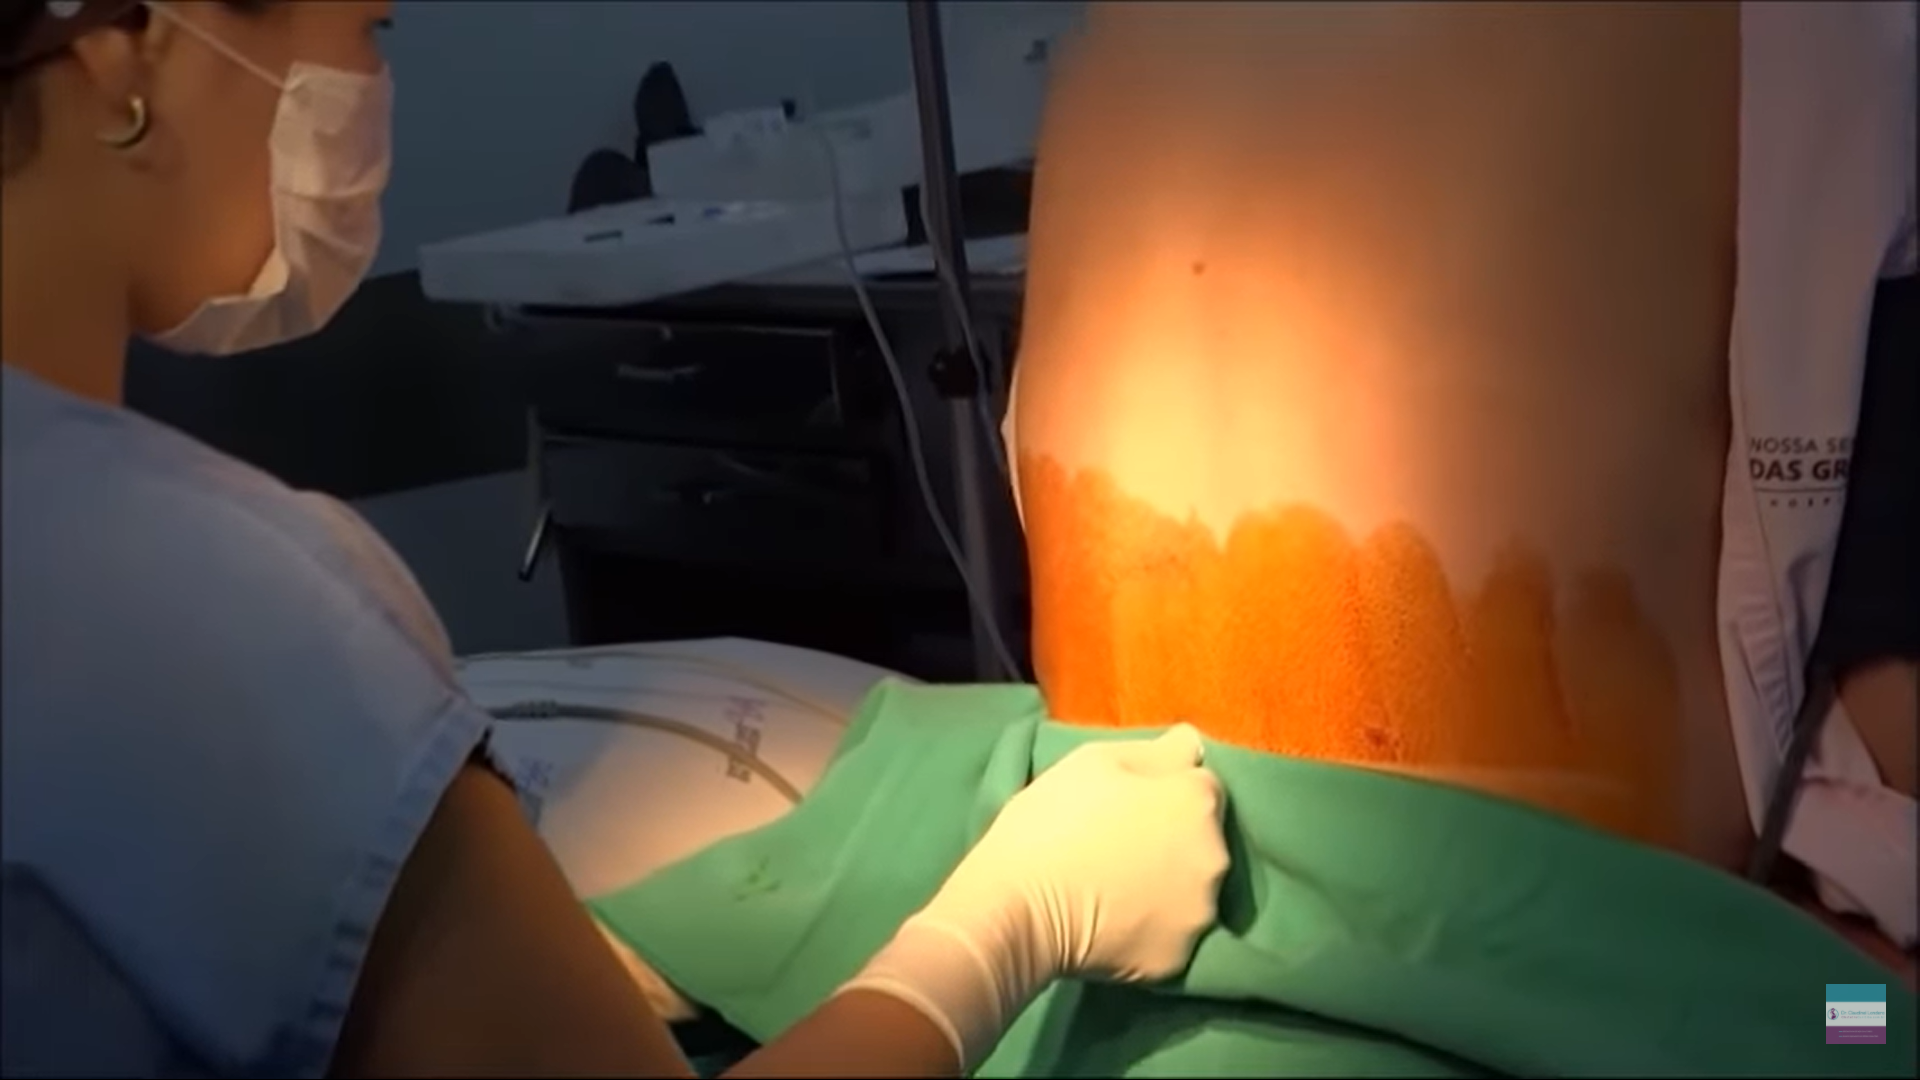
\includegraphics[width=0.6\linewidth]{capitulos/figuras/0.marcacaoPonto.png}
    \caption{Palpação para determinação do ponto de inserção da agulha \cite{Londero2018}.}
    \label{fig:marcacaoPonto}
\end{figure}

\begin{figure}[ht!]
    \centering
    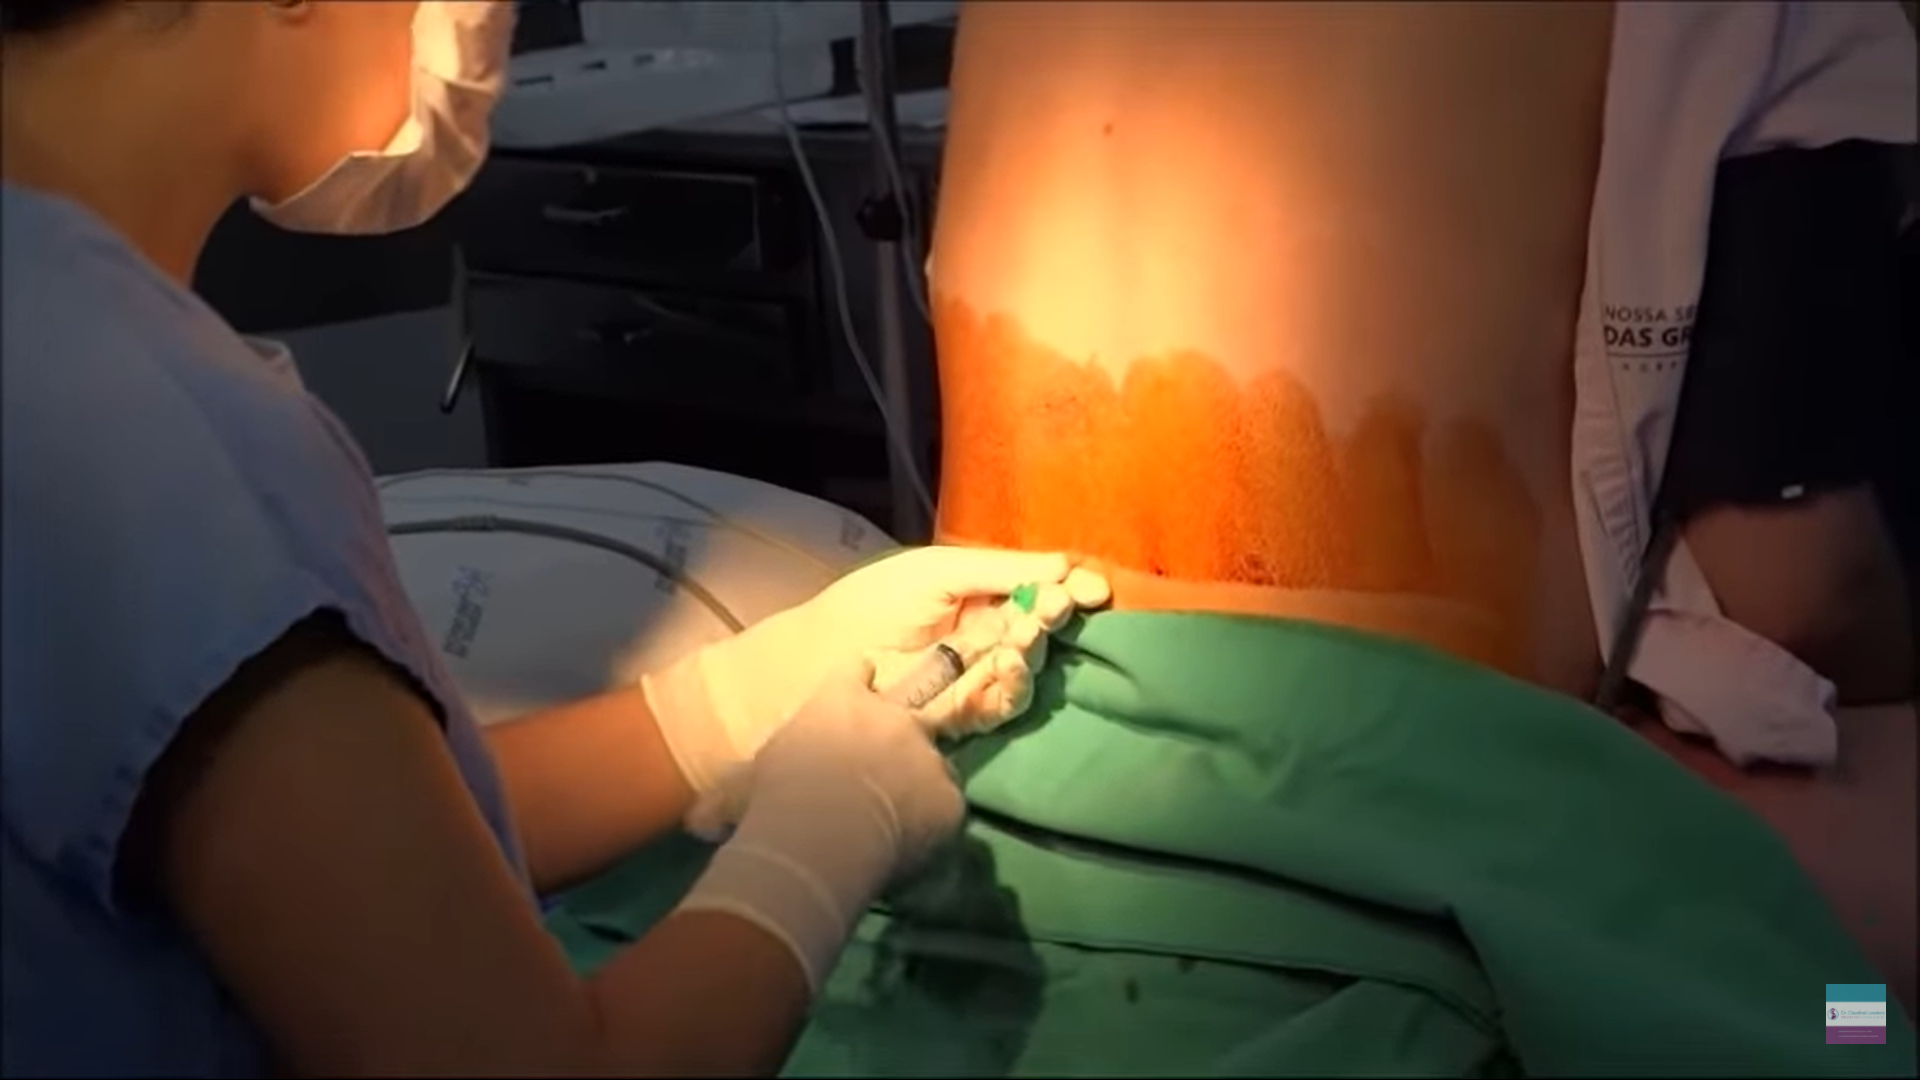
\includegraphics[width=0.6\linewidth]{capitulos/figuras/1.AnestesiaLocal.png}
    \caption{Aplicação da anestesia local \cite{Londero2018}.}
    \label{fig:anestesiaLocal}
\end{figure}

\begin{figure}[ht!]
    \centering
    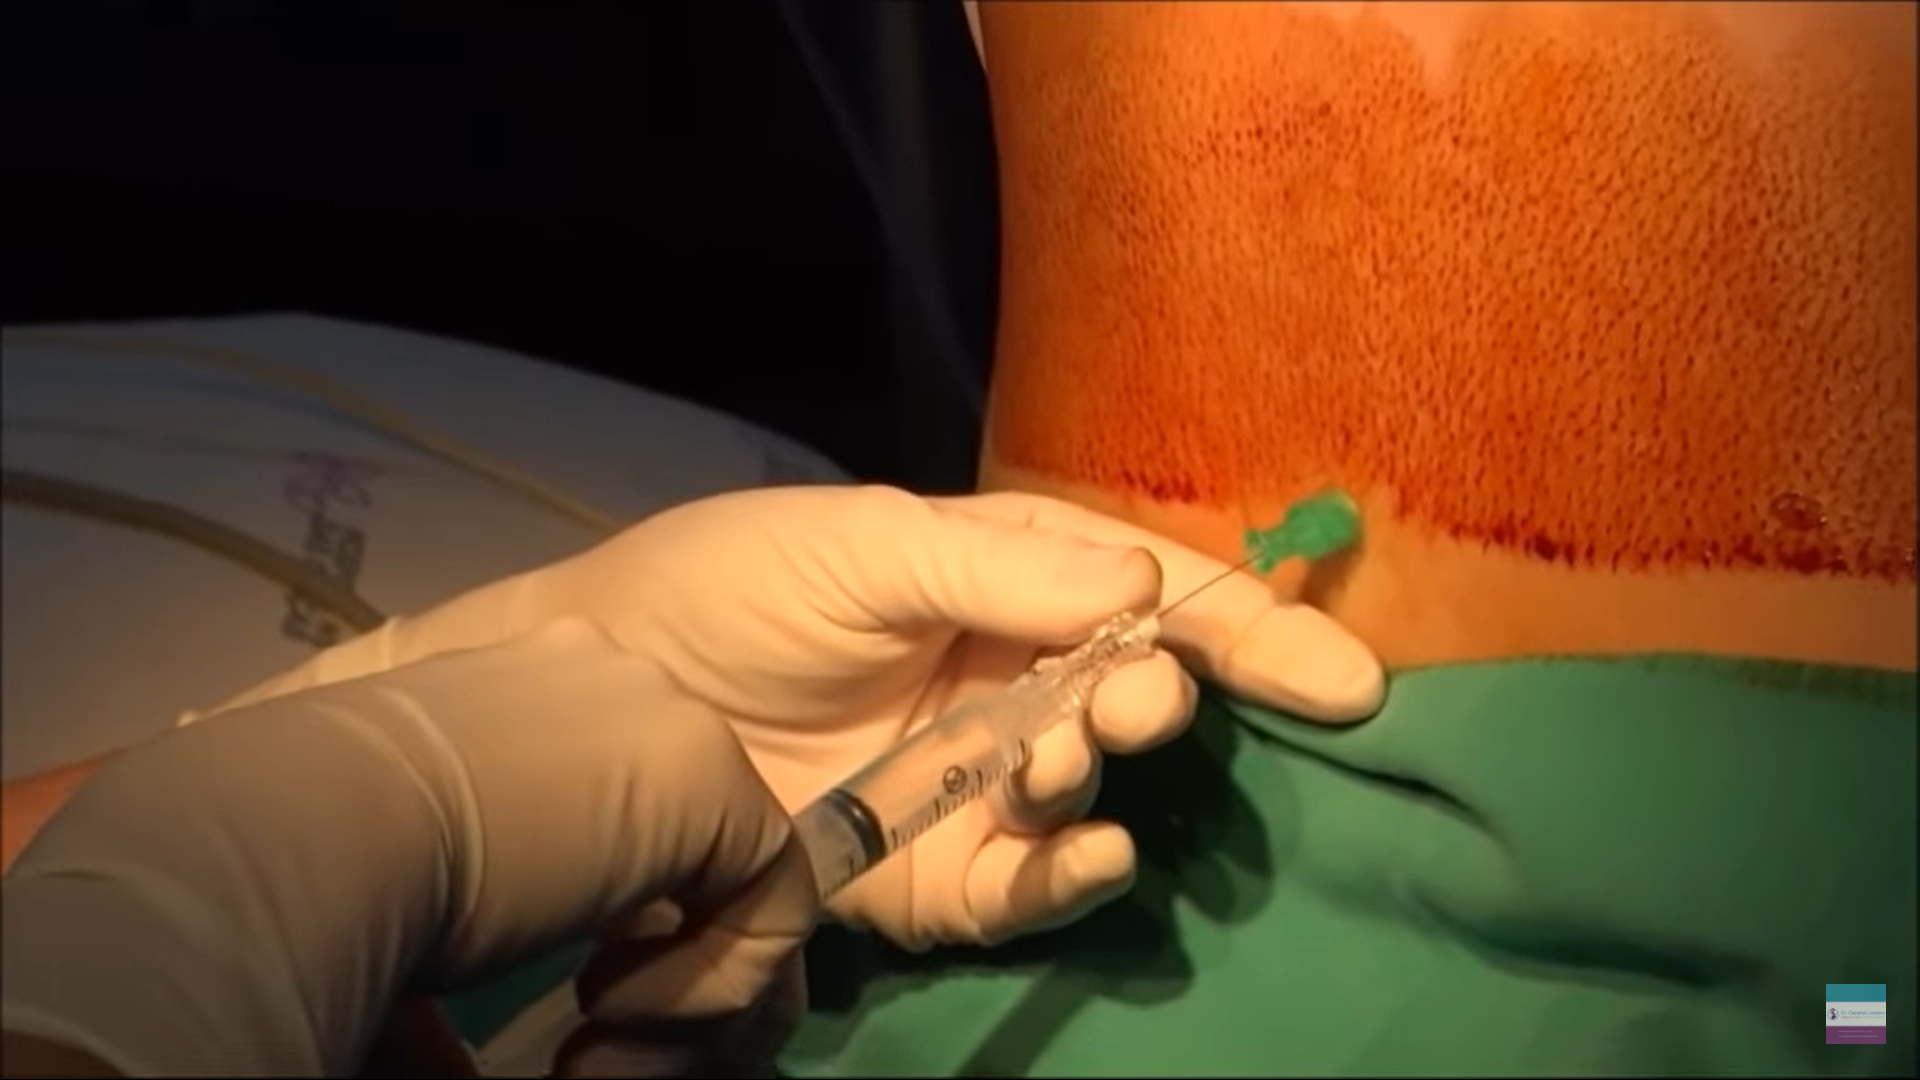
\includegraphics[width=0.6\linewidth]{capitulos/figuras/4.InjecaoAnestesico.png}
    \caption{Injeção do liquido anestésico no espaço subaracnóideo  \cite{Londero2018}.}
    \label{fig:injecaoAnestesico}
\end{figure}

Após a finalização dos procedimentos de preparação é escolhida a área onde será feita a punção através do toque da mão do médico (exemplo retirado de video na Figura~\ref{fig:marcacaoPonto}) na crista ilíaca do paciente \cite{Helayel2010,Isaacs2015}. Uma vez escolhido este ponto é feita a injeção de anestésico local (Figura~\ref{fig:anestesiaLocal}) para reduzir o desconforto na área próxima à punção \cite{Sedicias2018} Após a anestesia local é feita a inserção da agulha de punção tanto no caso da peridural como na raqui.

Existem duas principais abordagens de inserção da agulha para efetuação das anestesias regionais. Estão são denominadas mediana (do inglês \textit{midline}) e paramediana (do inglês \textit{paramedian}). A abordagem mediana é utilizada com mais frequência (96\%) \cite{Wantman2006}. Um dos motivos para o maior uso da abordagem mediana é a ausência de vasos sanguíneos no caminho da agulha nesta abordagem \cite{Bapat2015}. A abordagem paramediana é mais recomendada para pacientes idosos \cite{Ahsan-ul-Haq2005} por motivos de modificação degenerativa da coluna vertebral \cite{Boon2003} e calcificação dos ligamentos interespinhoso e supraespinhoso \cite{Wantman2006}. A abordagem paramediana também pode ser mais viável que a mediana em pacientes obesos pela dificuldade na identificação da crista ilíaca nestes pacientes. Isto por que a camada de gordura faz com que a linha média seja mais difícil de localizar através do toque do médico \cite{N.2013}. Na abordagem mediana a agulha é inserida na linha média da coluna vertebral. Na paramediana existe certa angulação entre a linha da coluna e a inserção da agulha. As duas abordagens podem ser observadas no corte transversal da coluna na Figura~\ref{fig:abordagensInsercaoAgulha}. 

\begin{figure}[ht!]
    \centering
    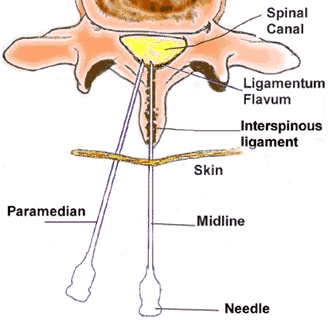
\includegraphics[width=0.6\linewidth]{capitulos/figuras/paramedian-midline-MedBroadcast-Tiff.png}
    \caption{Ilustração da abordagem mediana e paramediana para inserção de agulha \cite{MedBroadcast2018}.}
    \label{fig:abordagensInsercaoAgulha}
\end{figure}

\subsection{Anestesia Raquidiana}

Neste tipo de anestesia, uma agulha de pequeno calibre é inserida nas costas do paciente até atingir o espaço subaracnóideo (localizado após a dura-máter), dentro da coluna espinhal. Em seguida, um anestésico é injetado dentro do líquido cérebro espinhal (\textit{líquor}), produzindo dormência temporária e relaxamento muscular (Figura~\ref{fig:injecaoAnestesico}). Anestesias raquidianas são aplicadas de forma mais frequente em espaços intervertebrais abaixo da segunda vértebra lombar (L2), normalmente entre a L3 e L4 \cite{Wikipedia2019, Londero2018}. A Figura~\ref{fig:camadasPuncaoLombar} ilustra em um corte sagital da coluna as diferentes camadas que são cruzadas por uma agulha durante o procedimento de punção lombar até chegar ao espaço subaracnóideo. Considerando as duas abordagens de inserção da agulha (mediana e paramediana) as camadas onde a agulha pode passar desde a pele até o espaço subaracnóideo são: gordura subcutânea, músculo, ligamento supraespinhoso, ligamento interespinhoso, ligamento amarelo (\textit{flavum}), espaço epidural e dura-máter. O processo espinhoso que também aparece entre a pele e o espaço subaracnóideo na Figura~\ref{fig:camadasPuncaoLombar} não foi listado, pois, por ser uma camada de osso, ela não é perfurada pela agulha e sim uma camada intransponível em relação ao processo de punção.

\begin{figure}[ht!]
    \centering
    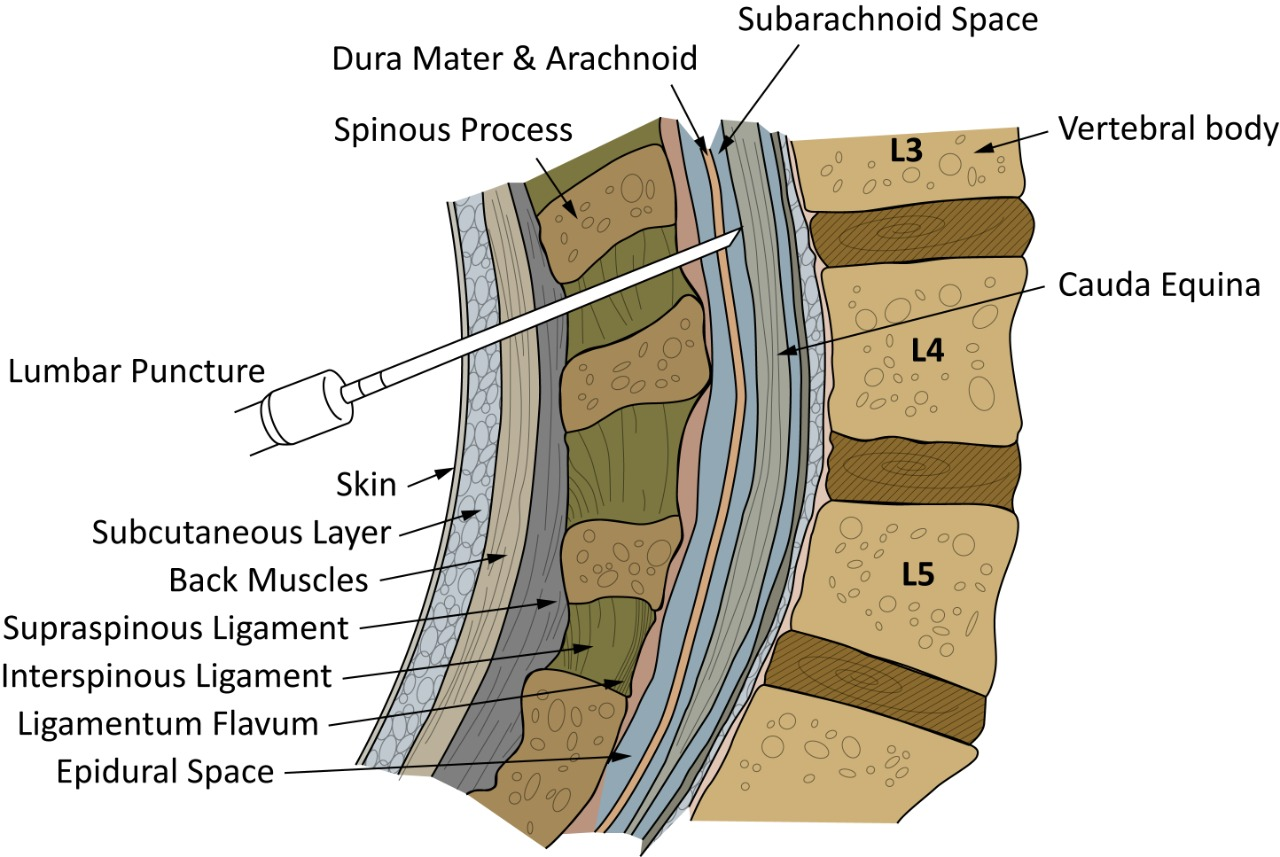
\includegraphics[width=0.6\linewidth]{capitulos/figuras/lumbar.puncture.tisssues.jpeg}
    \caption{Camadas cruzadas pela agulha numa punção lombar.}
    \label{fig:camadasPuncaoLombar}
\end{figure}

A ação do anestésico dentro da coluna espinhal é a de bloquear os nervos que passam pela coluna lombar, fazendo com que os estímulos dolorosos vindos de membros inferiores e do abdômen não cheguem ao cérebro. A raquianestesia é muito usada para procedimentos ortopédicos de membros inferiores assim como na região abdominal e cirurgias obstétricas de parto normal e cesarianas \cite{Pinheiro2018}.

A grande vantagem da anestesia raquidiana em relação a peridural é que nesta é necessário o uso de uma pequena quantidade de anestésico local. Esta característica reduz consideravelmente o risco de intoxicação por meio do elemento anestésico. Por outro lado a maior desvantagem no uso deste tipo de anestesia está na dor de cabeça que os pacientes sentem após a perfuração da dura-máter. Este sintoma é causado pela lesão na dura-máter que pode permanecer aberta por alguns dias após o procedimento, provocando perda do \textit{líquor} do espaço subaracnóideo. Com o uso de agulhas de menor diâmetro a incidência desta dor de cabeça foi consideravelmente reduzida \cite{INFOESCOLA2018}. 

\section{Realidade Virtual}

A \acrlong{RV} está presente quando se usa a tecnologia para criar a ilusão de que se está em um ambiente que não está lá ou não existe. Ela é uma aproximação da realidade experimentada por nós através dos nossos sentidos e sistemas de percepção. A nossa percepção da realidade vem através dos nossos sentidos. Portanto, uma vez apresentando aos sentidos às informações esperadas, sendo estas reais ou não, a nossa percepção da realidade irá se guiar por estes estímulos. Os sentidos mais comuns são visão, olfato, paladar, audição e tato. Porém também possuímos outros sentidos que afetam as nossas percepções do mundo, como por exemplo: o senso de equilíbrio, o sentimento de forças, pesos e deslocamentos sentidos por nossos membros \cite{VRS2018}.

Atualmente, a chamada \acrfull{RV} utiliza um computador para criar um ambiente virtual tridimensional. A intenção é a de simular uma realidade apresentando os elementos desejáveis para os sentidos do usuário, visando cumprir um objetivo através da interação de um ou mais usuários com este ambiente. Estes usuários se tornam parte deste ambiente virtual, total ou parcialmente, podendo manipular objetos ou executar um conjunto de ações \cite{VRS2018}.

A \acrshort{RV} possui uma série de usos sociais como, por exemplo, o tratamento de fobias. Há trabalhos para aracnofobia \cite{Carlin1997}, para aicmofobia ou medo de agulhas \cite{Galoustian2018}, para aerofobia ou medo de voar \cite{Rothbaum2006}, para acrofobia ou medo de altura \cite{Edwards2018} ou de forma mais geral para o medo e a ansiedade \cite{Goldman2017}. A Figura~\ref{fig:medoAltura} ilustra a aplicação para tratamento da acrofobia. Em primeiro plano a usuária com os óculos de realidade virtual e no segundo plano o ambiente virtual simulando ambientes de escadas e plataformas com fundo transparente.

\begin{figure}[ht!]
    \centering
    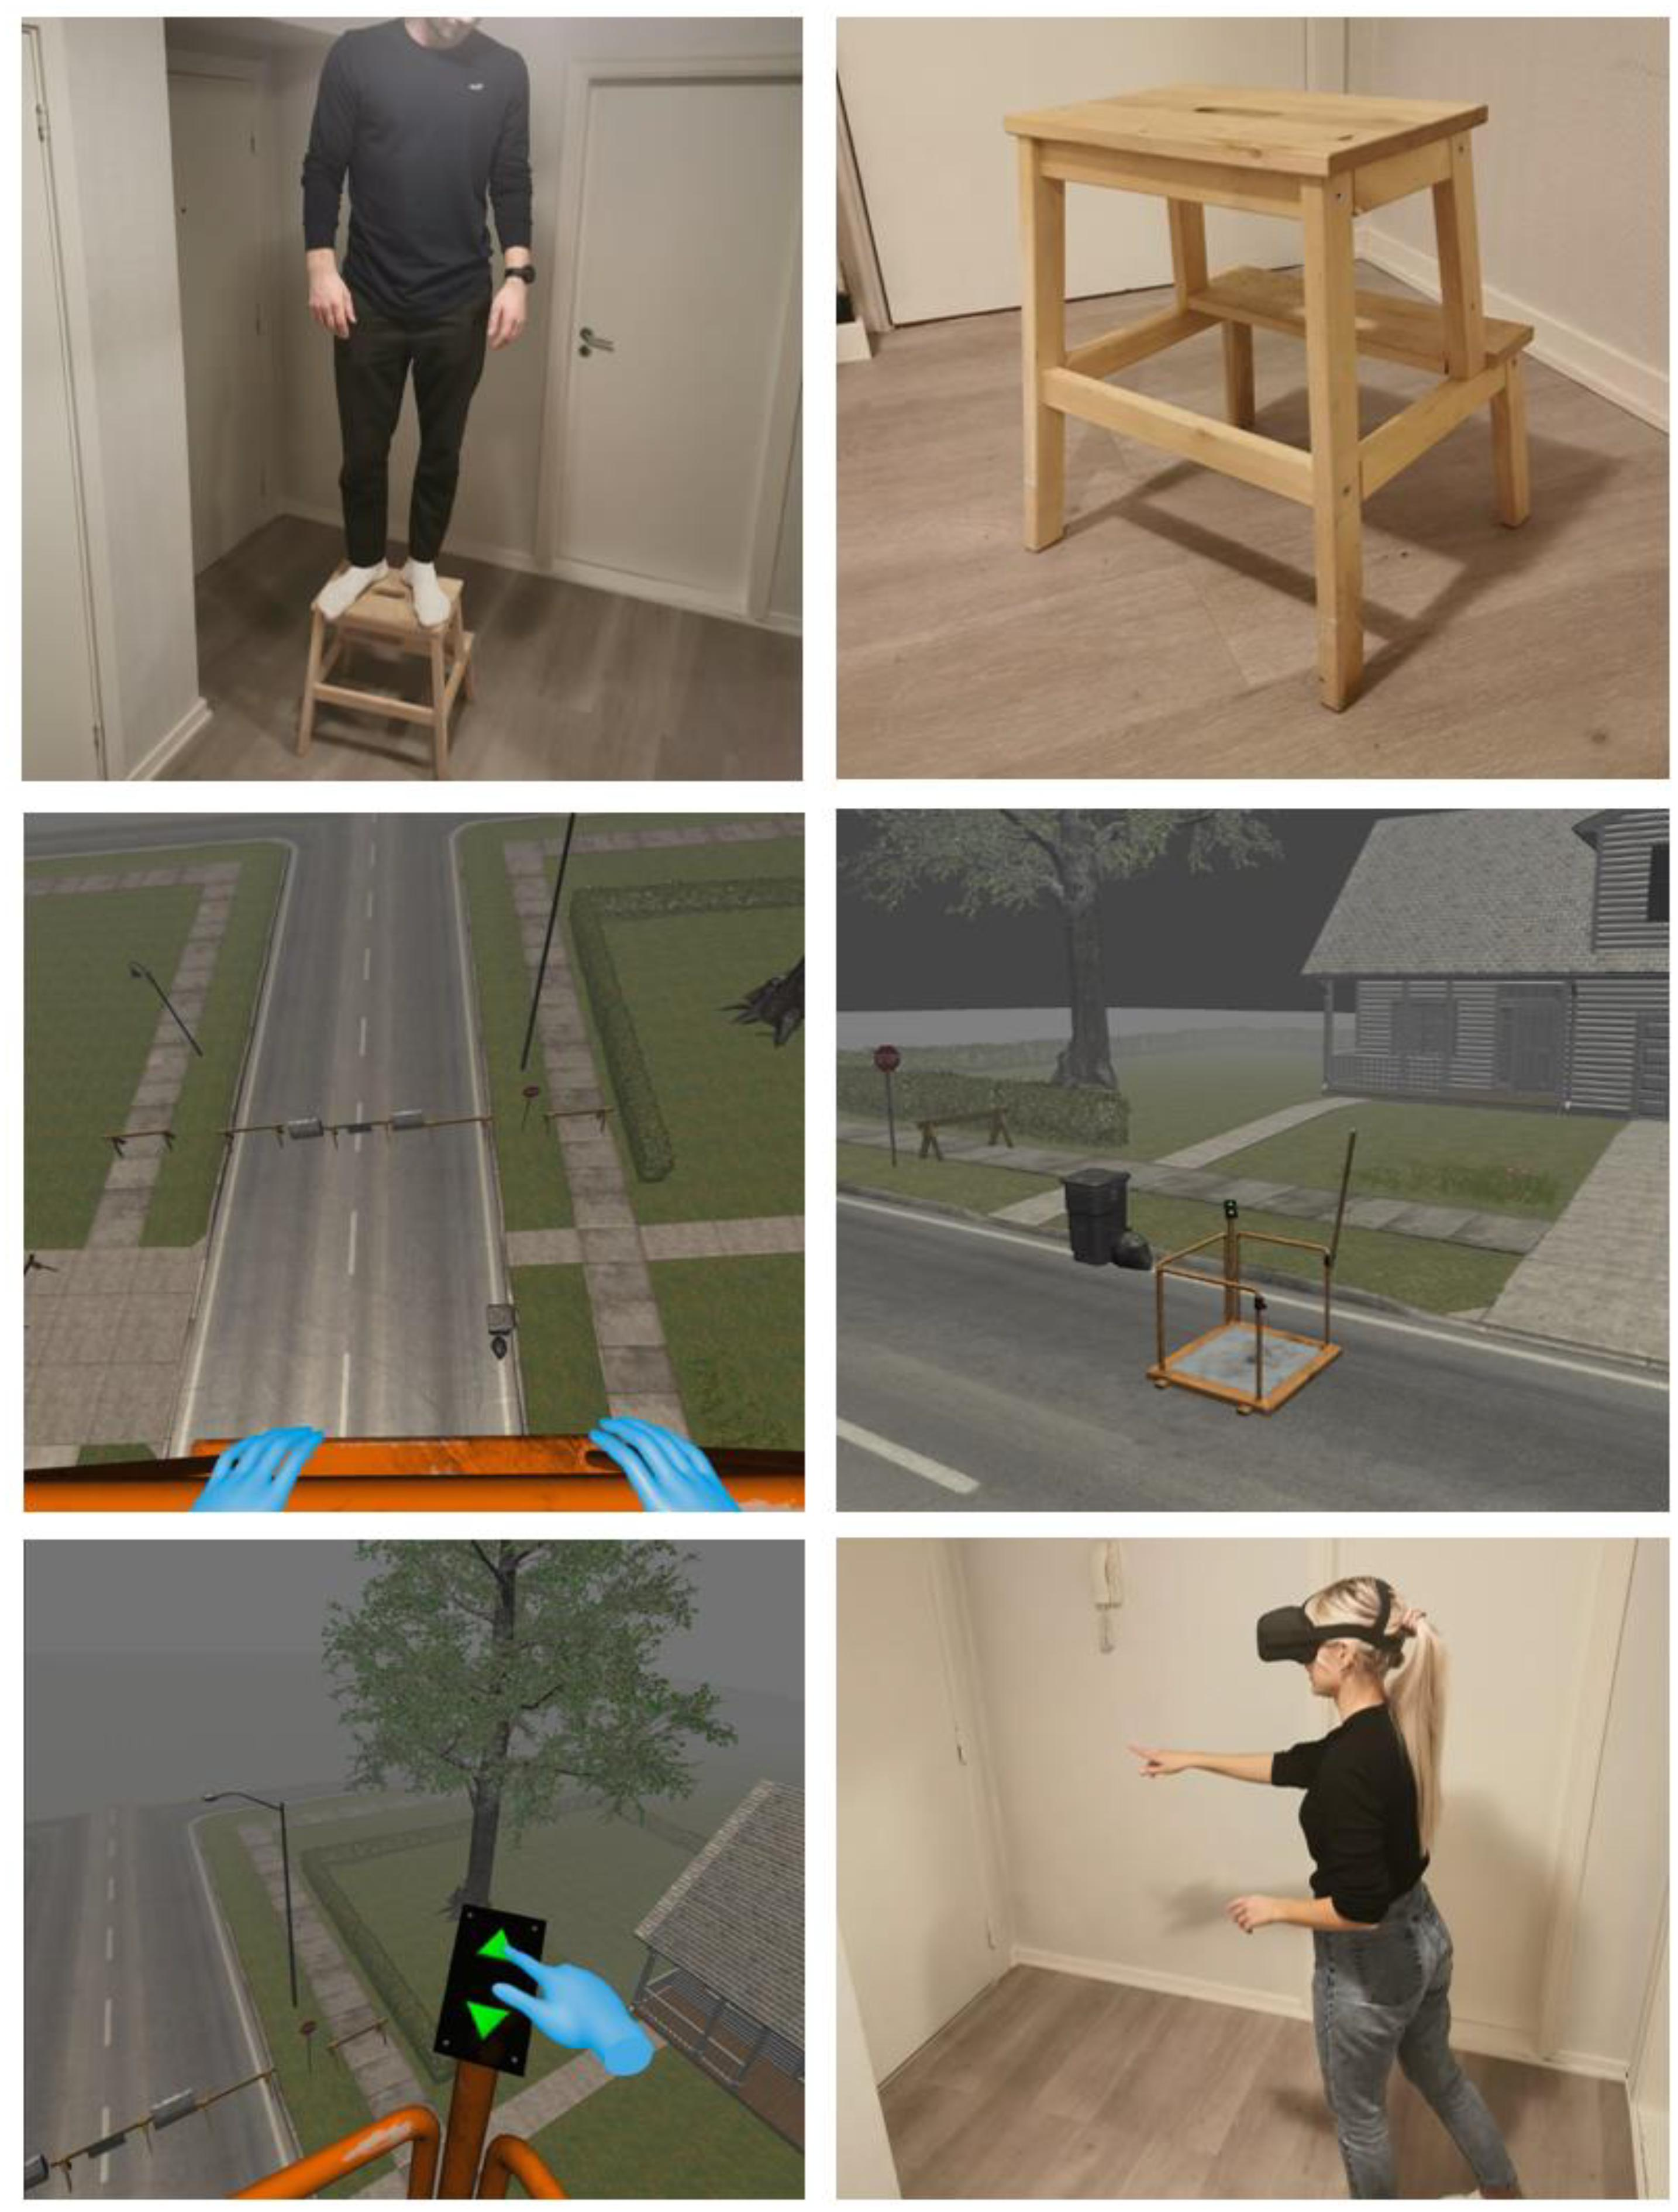
\includegraphics[width=0.6\linewidth]{capitulos/figuras/fear_of_heights.jpg}
    \caption{Exemplo de aplicação que usa \acrshort{RV} no tratamento da acrofobia \cite{Edwards2018}.}
    \label{fig:medoAltura}
\end{figure}

A indústria do entretenimento através de filmes e jogos provocou uma grande evolução de técnicas de \acrshort{RV} que posteriormente foram aplicadas em áreas mais “sérias” como o desenvolvimento pessoal e treinamento \cite{Ma2011, Prensky2001, Smith2011}. Na prática a \acrshort{RV} deve ser considerada como uma possibilidade sempre que o que se deseja fazer é muito perigoso, caro ou impraticável de ser realizado concretamente. Por conta destas características ela é muito usada nas áreas da educação, da saúde e militar \cite{VRS2018}. Conforme a tecnologia que permite a criação e simulação de ambientes virtuais se torna mais barata, mais aplicações são criadas com o uso destas ferramentas.

\section{Dispositivos Hápticos}

O termo \textit{haptics} é usado para descrever a ciência que estuda e simula a pressão, textura, vibração e outras sensações biológicas relacionadas ao toque. A sensação do toque se origina em estímulos mecânicos, elétricos, térmicos ou químicos na pele \cite{Burdea1996}. O tato não está localizado numa região específica do corpo como os demais sentidos. Ele está distribuído por todo o corpo através do órgão sensorial do toque, nossa pele, articulações, músculos e tendões. O senso do toque se divide em duas sensações: cinética e tátil. Forças e torques são sensações cinéticas que sentimos nos músculos, tendões e articulações. Já as sensações táteis como pressão, deformação e vibração são sentidas por mecano receptores que possuímos na nossa pele \cite{Culbertson2018}. 

Os primeiros dispositivos hápticos foram originados dos braços robóticos usados para o controle remoto de robôs \cite{Zurawski2005} As aplicações de tecnologias hápticas são muito variadas envolvendo, por exemplo, projetos de engenharia e aplicações de manufatura \cite{Sharma2001}, entretenimento (videogames e filmes), celulares, relógios inteligentes e até mesmo a indústria automobilística \cite{Smith2019}. Estes dispositivos possuem elementos mecânicos de entrada e saída para interação com o usuário. Uma ou mais partes do dispositivo em contato com o usuário são monitorados no espaço físico e o dispositivo oferece como retorno força e torque. Desta forma um canal bidirecional de interação entre o ambiente virtual e o usuário é criado \cite{Coles2011}. Estes dispositivos estão sendo cada vez mais utilizados hoje em dia tanto pela evolução da sua tecnologia como pela diminuição dos preços. Com o avanço da tecnologia estes dispositivos estão se tornando cada vez mais flexíveis representando mais fielmente os movimentos. Isto ocorre  através do uso de conceitos de restrição parcial a movimentos, deslocamentos e da inclusão de mais graus de liberdade, \textit{\acrfull{DoF}}. 

O número de graus de liberdade de um dispositivo háptico se refere ao número de maneiras diferentes em que este pode se mover ou criar forças. Como exemplo, dispositivos com 3 graus de liberdade podem rastrear posições e criar forças ao serem movidos nas direções: direita-esquerda, frente-trás e cima-baixo \cite{HAPTICSHOUSE2019}. O principal objetivo no uso destes dispositivos é o aumento da sensação de imersão em um ambiente de realidade virtual. 

Em relação à área médica, os dispositivos hápticos vem sendo utilizados na maioria dos trabalhos de simulação de procedimentos médicos \cite{Coles2011,Escobar-Castillejos2016}. Eles são usados para simular o uso de ferramentas em cirurgias e ajudaram a impulsionar o sucesso das práticas em simuladores virtuais. Isto aconteceu ao proporcionar o controle dos graus de liberdade de deslocamentos, a restrição aos movimentos e as respostas às atitudes do usuário como forças de reação ou \textit{feedback} \cite{Gerovich2004}. Estes dispositivos eletromecânicos existem nas mais diversas formas e são adaptados para uma grande variedade de procedimentos médicos como, por exemplo, no treinamento de laparoscopia \cite{Srinivasan2004}, biopsia de próstata \cite{Sclaverano2009}, cirurgia de fígado \cite{Mastmeyer2016}, exames de mama \cite{Brazil2017,Jeon2010,Ribeiro2014,Solanki2010}, simulação de apalpação \cite{Ribeiro2016} e punções epidurais \cite{N.2013, Brazil2018}. Alguns sistemas usam mais de um háptico como em punções de agulha guiadas por ultrassom que usam um equipamento para simular a agulha e outro para o ultrassom \cite{Ni2011,Vidal2008}. Outros chegam a fazer o uso de três dispositivos como o PalpSim de forma a simular o toque das mãos do usuário num paciente virtual \cite{Coles2011b}. 

Culbertson et al. identificaram como 3 as principais categorias de sistemas hápticos: compreensíveis, vestíveis e palpáveis. Um exemplo visual destes tipos pode ser visto na Figura 6. Os sistemas compreensíveis são dispositivos tipicamente cinéticos (\textit{feedback} de força) que normalmente possuem uma base fixa e permitem ao usuário empurrar e ser empurrado de volta. Sistemas vestíveis são tipicamente táteis montados nas mãos ou em outras partes do corpo e provocam sensações diretamente na pele. Os sistemas palpáveis são dispositivos de encontro que permitem ao usuário explorar toda a superfície \cite{Culbertson2018}. Os dispositivos a serem explorados aqui são os de sistemas compreensíveis. Estes foram os tipos de hápticos utilizados nos simuladores computacionais relacionados ao tema desta tese (seção 0) assim com nos diversos outros simuladores médicos estudados e citados nesta seção. Ribeiro et al. fizeram uma revisão sobre dispositivos usados na simulação de procedimentos que envolvem o toque da mão do médico para identificação de características e anormalidades sob a pele \cite{Ribeiro2016}. Os autores analisaram 57 trabalhos e mais da metade fez uso dos dispositivos da família \textit{Phantom}. Os dispositivos desta família serão listados na seção ===== 3 ======.

===== FIGURA ====

Nas figuras Figura 7, Figura 8, Figura 9 e Figura 10 os dispositivos aparecem representados ordenados pelas suas complexidades i.e. dos mais simples (mais antigos e com menos recursos) aos mais avançados (mais novos). Todos estes dispositivos são exemplos de sistemas tipicamente cinéticos. Os mais novos possibilitam maior número de graus de liberdade para os movimentos assim como possibilitam mais forças e momentos de reação. O Novint Falcon ® (Figura 7), lançado em 2007, tem como interface com o usuário uma esfera onde o usuário deve colocar os dedos da mão para fazer os movimentos no caso do seu uso mais comum. No que diz respeito à liberdade de movimento este mecanismo proporciona uma interação 3D com o computador no lugar da interação 2D proporcionada pelo mouse. Ele possui 3 graus de liberdade de movimento e de forças. Nesta esfera existem quatro botões para interação e existem sensores para determinar a posição do cursor e motores para controlar as forças a serem transmitidas para o usuário. Existem versões onde a esfera é substituída, por exemplo, por um dispositivo semelhante a uma pistola para que o dispositivo seja usado em jogos de tiros de primeira pessoa \cite{VRS2017}. 

===== FIGURA ====

Os hápticos da família \textit{Phantom Geomagic Touch} ® (Figura 8) e \textit{Geomagic Touch} X ® (Figura 9) apresentam uma peça que simula uma caneta para manipulação do usuário da mesma forma que a esfera no dispositivo da Figura 7. Nas canetas também existem botões para interação e da mesma forma estas também são substituíveis por partes com formas mais adequadas ao procedimento que estas pretendem simular. O dispositivo \textit{Geomagic Touch} X ® possui a mesma liberdade de movimento do \textit{Geomagic Touch} ®, porém possibilita \textit{feedback} de reações maiores. Ambos apresentam 6 graus de liberdade de movimento e 3 graus de liberdade no retorno de forças. Estes dispositivos, portanto mapeiam a posição 3D e orientação, mas somente apresentam \textit{feedback} de forças direcionais \cite{Forsslund2013}.

===== FIGURA ====

===== FIGURA ====

O \textit{Phantom Premium} ® (Figura 10) está disponível nas versões \textit{Premium} 1.0, \textit{Premium 1.5} e 1.5/HF, e \textit{Premium} 3.0. Estas evoluem não só o \textit{feedback} de reações como também os graus de liberdade dos movimentos. Enquanto o \textit{Phantom Premium} 1.0 ® simula o movimento do giro do pulso na mão o \textit{Phantom Premium} 3.0 ® possibilita uma amplitude que simula os graus de liberdade de movimento de todo o braço humano desde o ombro \cite{3DSystems2018}. Este dispositivo possui 6 graus de liberdade tanto para movimento como retorno de forças o que o torna simétrico no número de sensores e motores (atuadores). São computadas forças e torques tanto da posição como da orientação deste dispositivo. Esta característica tem uma forte influencia no alto custo associado a este tipo de dispositivo \cite{Forsslund2013}.

===== FIGURA ====

=========

\section{Modelagem de tecidos}

Um dos passos necessários para construção de um ambiente virtual para treinamento de anestesia epidural e raquianestesia é a criação de pacientes virtuais. Um importante aspecto da modelagem destes pacientes é como eles aparecem na tela da aplicação. Outro aspecto importante na simulação é ter uma estimativa da espessura dos tecidos envolvidos nestes tipos de anestesia. Para isto é necessária à modelagem do tamanho de todas as camadas de tecido pelos quais as agulhas passam para execução destes procedimentos. Uma ilustração destes tecidos que vão desde a pele até a dura-máter pode ser vista na Figura 3. Nesta seção são descritos trabalhos relacionados com a modelagem da distância entre a pele e a dura-máter.

Na Tabela 2 são listadas as varáveis de entrada e saída dos métodos estudados nesta seção. Esta tabela exibe também as unidades destas variáveis que serão utilizadas em todo este trabalho.

===== TABELA ====

Muitos trabalhos buscam relacionar a distância que vai da superfície externa da pele até o espaço epidural (DEE) com as demais variáveis da Tabela 2. A grande maioria dos trabalhos indica uma forte relação da DEE com o IMC \cite{Adegboye2017, Galbraith2018}. Estes dois trabalhos não fazem separação dos grupos populacionais por idade, sexo ou etnia, e usaram populações respectivamente de n=120 e n=317 pessoas entre homens e mulheres.

Os trabalhos citados a seguir analisaram somente ou de forma separada grupos de mulheres grávidas. Como este é o foco deste trabalho só serão comentadas aqui as conclusões referentes a estes grupos. Todos os trabalhos a seguir encontraram influencia do IMC na determinação da DEE, mas além desta relação também foram encontradas outras combinações em cada trabalho. O grupo étnico/populacional do individuo foi observado em conjunto com o IMC em \cite{Sharma2011} estudo feito no Reino Unido. A idade foi observada em conjunto com o IMC num estudo em pacientes americanas em Michigan, EUA \cite{Clinkscales2007}. A altura, massa, idade e IMC foram observados como relevantes em um estudo em pacientes da Índia \cite{Hazarika2016}. Estes dois últimos trabalhos construíram equações de regressão linear para determinação da DEE para grupos de parturientes conforme pode ser visto na Tabela 3.

===== TABELA ====

Os autores em \cite{Sharma2011} no lugar das equações apresentaram como resultado uma tabela com cinco pontos de cada par IMC x DEE para cada grupo populacional analisado. Estes dados podem ser vistos na Tabela 4. A definição dos grupos populacionais no estudo do Reino Unido (RU) em \cite{Sharma2011} foi: Brancas (população do Reino Unido, da Irlanda e qualquer outro grupo com cor de pele branca); Asiáticas ou Britânicas Asiáticas (população da Índia, Paquistão, Bangladesh ou qualquer outro grupo Asiático); Negras ou Britânicas negras (população de Africanas, Caribenhas ou outros grupos com cor da pele negra); e Chinesas e outros grupos étnicos (população da China, Japão, Malásia, Filipinas etc.). No grupo de nome Chinesas, além dos dados de pessoas desta origem moradoras do Reino Unido, foram considerados dados de Chinesas (n=70) de um hospital de Singapura.

===== TABELA ====

Na Tabela 5 é apresentado o tamanho da população utilizada nestes estudos e as identificações da origem dos dados do estudo, isto é, os grupos populacionais analisados. 

===== TABELA ====

A listagem dos tecidos entre a pele e a DEE e a relação dessa distância com o aumento de peso é comentada em \cite{Palmer1983}. Os autores concluem que com o aumento do peso/massa (do paciente) o tecido que sofre a maior variação é a gordura subcutânea.

Na seção = ==== é proposto o uso de dados de trabalhos comentados aqui para modelagem de tecidos de pacientes grávidas.

=========

Este capítulo apresentou uma fundamentação teórica sobre ====. Iniciou apresentando ==========. Logo em seguida o capítulo apresenta ====== e suas principais entidades e que estão relacionadas com a proposta desta tese. O capitulo finaliza apresentando os conceitos que envolvem ==== e seus principais elementos. O próximo capítulo oferece uma visão das pesquisas relacionadas ao tema desta tese e compara-as com as proposições que foram colocadas ao longo deste trabalho. Essas pesquisas tratam e ========== assim como de ===========.  %inclui novo capítulo

%\pagestyle{ruledheader} %inclui novo capítulo
%\chapter{Fundamentação Teórica} \label{cap:cap2}

Este Capítulo relaciona os conceitos e as tecnologias envolvidas no desenvolvimento do ambiente de treinamento proposto. 

\section{Anestesias Regionais}

Anestesias são atualmente usadas em diversos procedimentos cirúrgicos na medicina tradicional com o intuito de bloquear temporariamente a capacidade do cérebro de reconhecer um estímulo doloroso. Esta prática visa permitir a execução de procedimentos invasivos por parte do médico enquanto mantém o conforto e a tranquilidade do paciente. A anestesia regional é um procedimento usado em cirurgias onde o paciente pode permanecer acordado. Este tipo de anestesia bloqueia a dor em apenas uma determinada região do corpo, como um braço, uma perna ou toda região inferior do corpo, abaixo do abdômen \cite{Pinheiro2018}.

Os dois tipos de anestesias regionais mais usados são: anestesia raquidiana (ou raquianestesia, raqui), e anestesia peridural ou epidural. Estes dois tipos de anestesias também são conhecidas como anestesias de neuroeixo ou ainda bloqueio de neuroeixo \cite{Pinheiro2018}. Ambas podem ser aplicadas com pacientes sentados e inclinados para frente ou deitados de lado \cite{Anesclin2019}. 

\begin{figure}[ht!]
    \centering
    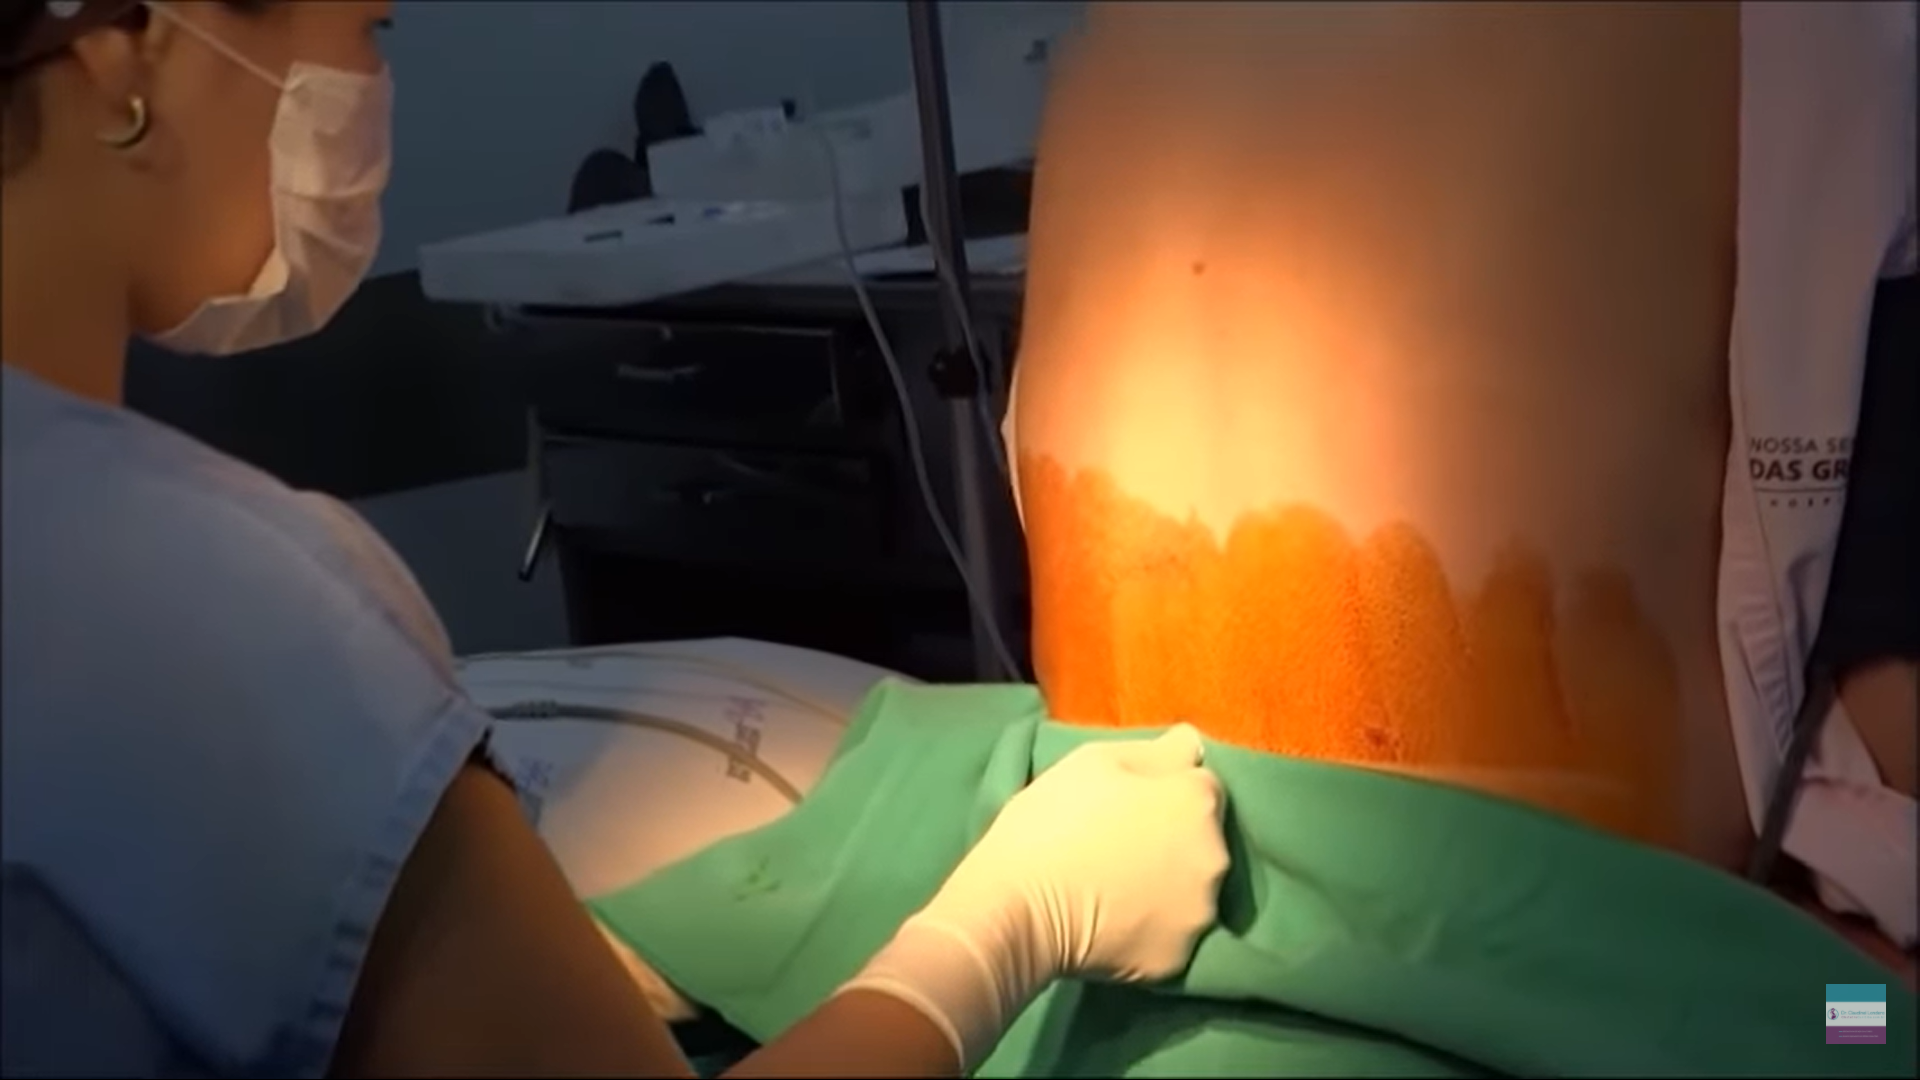
\includegraphics[width=0.6\linewidth]{capitulos/figuras/0.marcacaoPonto.png}
    \caption{Palpação para determinação do ponto de inserção da agulha \cite{Londero2018}.}
    \label{fig:marcacaoPonto}
\end{figure}

\begin{figure}[ht!]
    \centering
    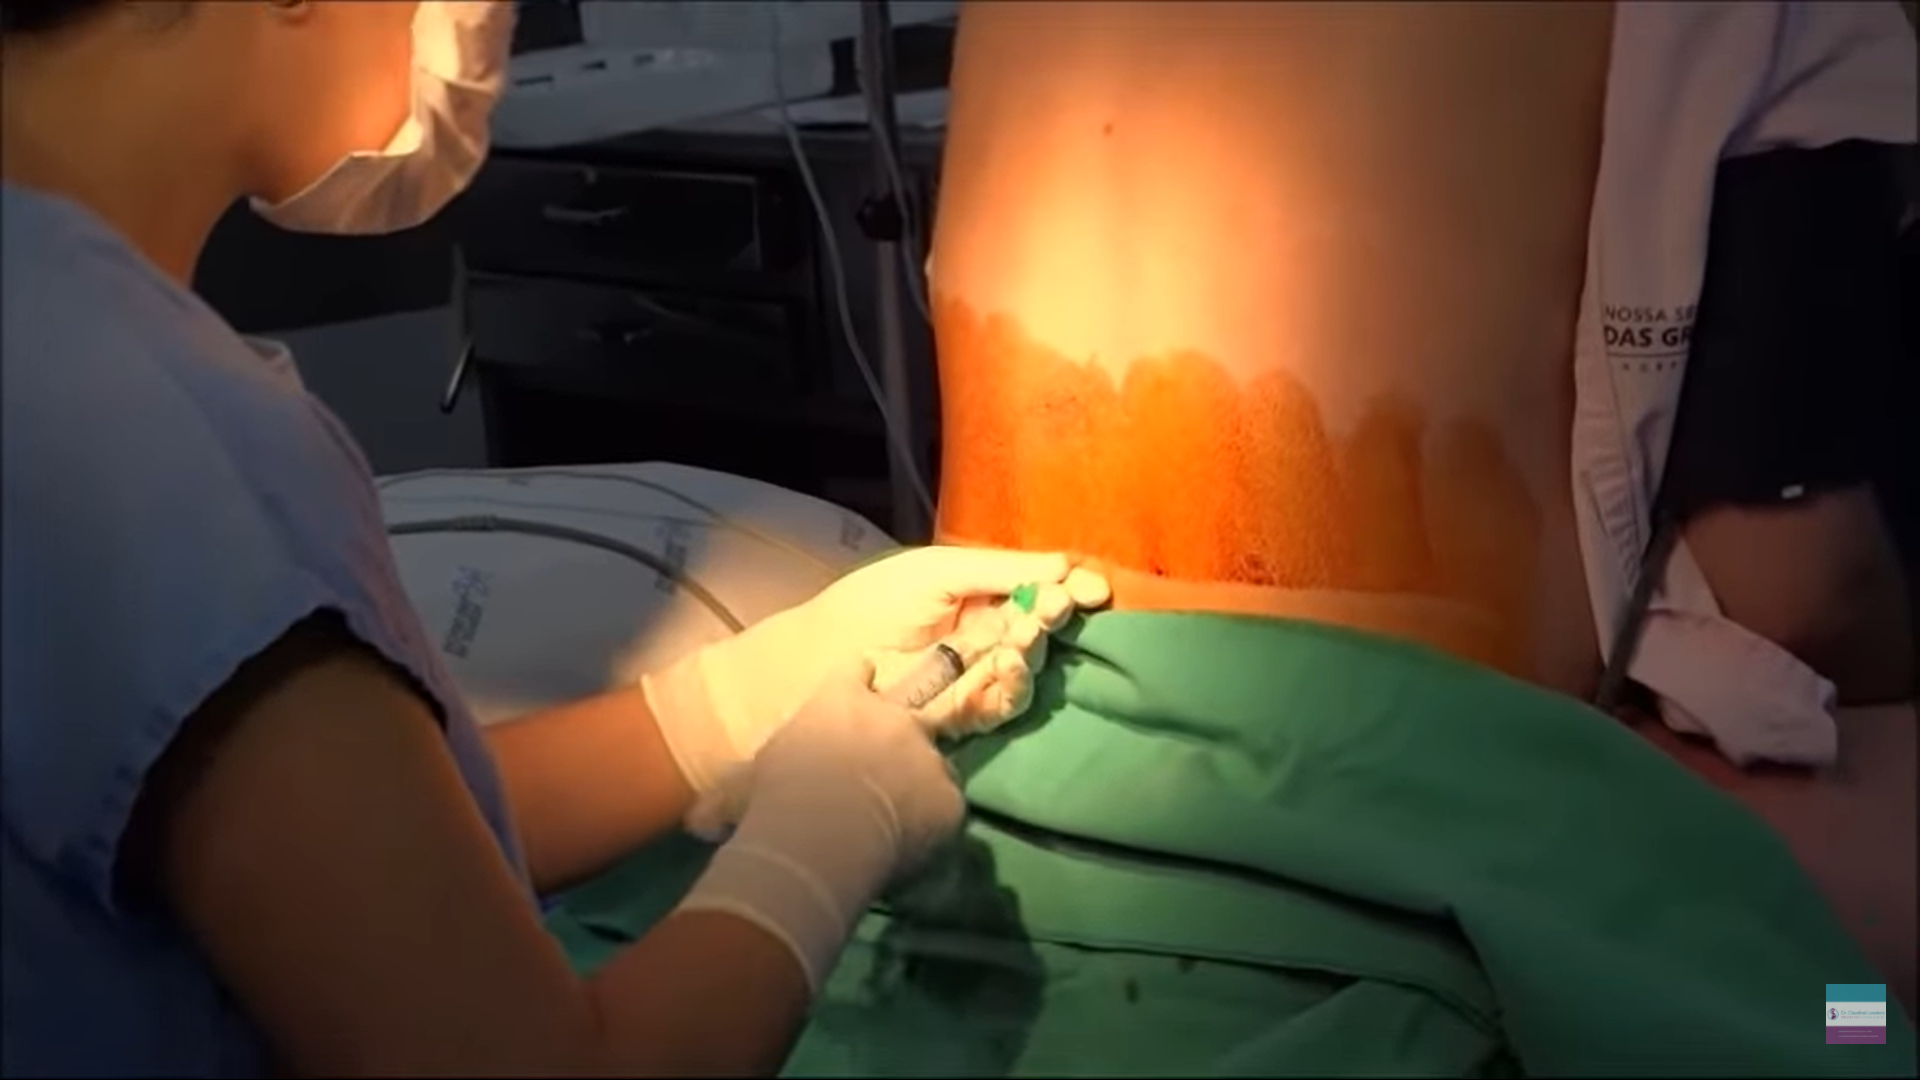
\includegraphics[width=0.6\linewidth]{capitulos/figuras/1.AnestesiaLocal.png}
    \caption{Aplicação da anestesia local \cite{Londero2018}.}
    \label{fig:anestesiaLocal}
\end{figure}

\begin{figure}[ht!]
    \centering
    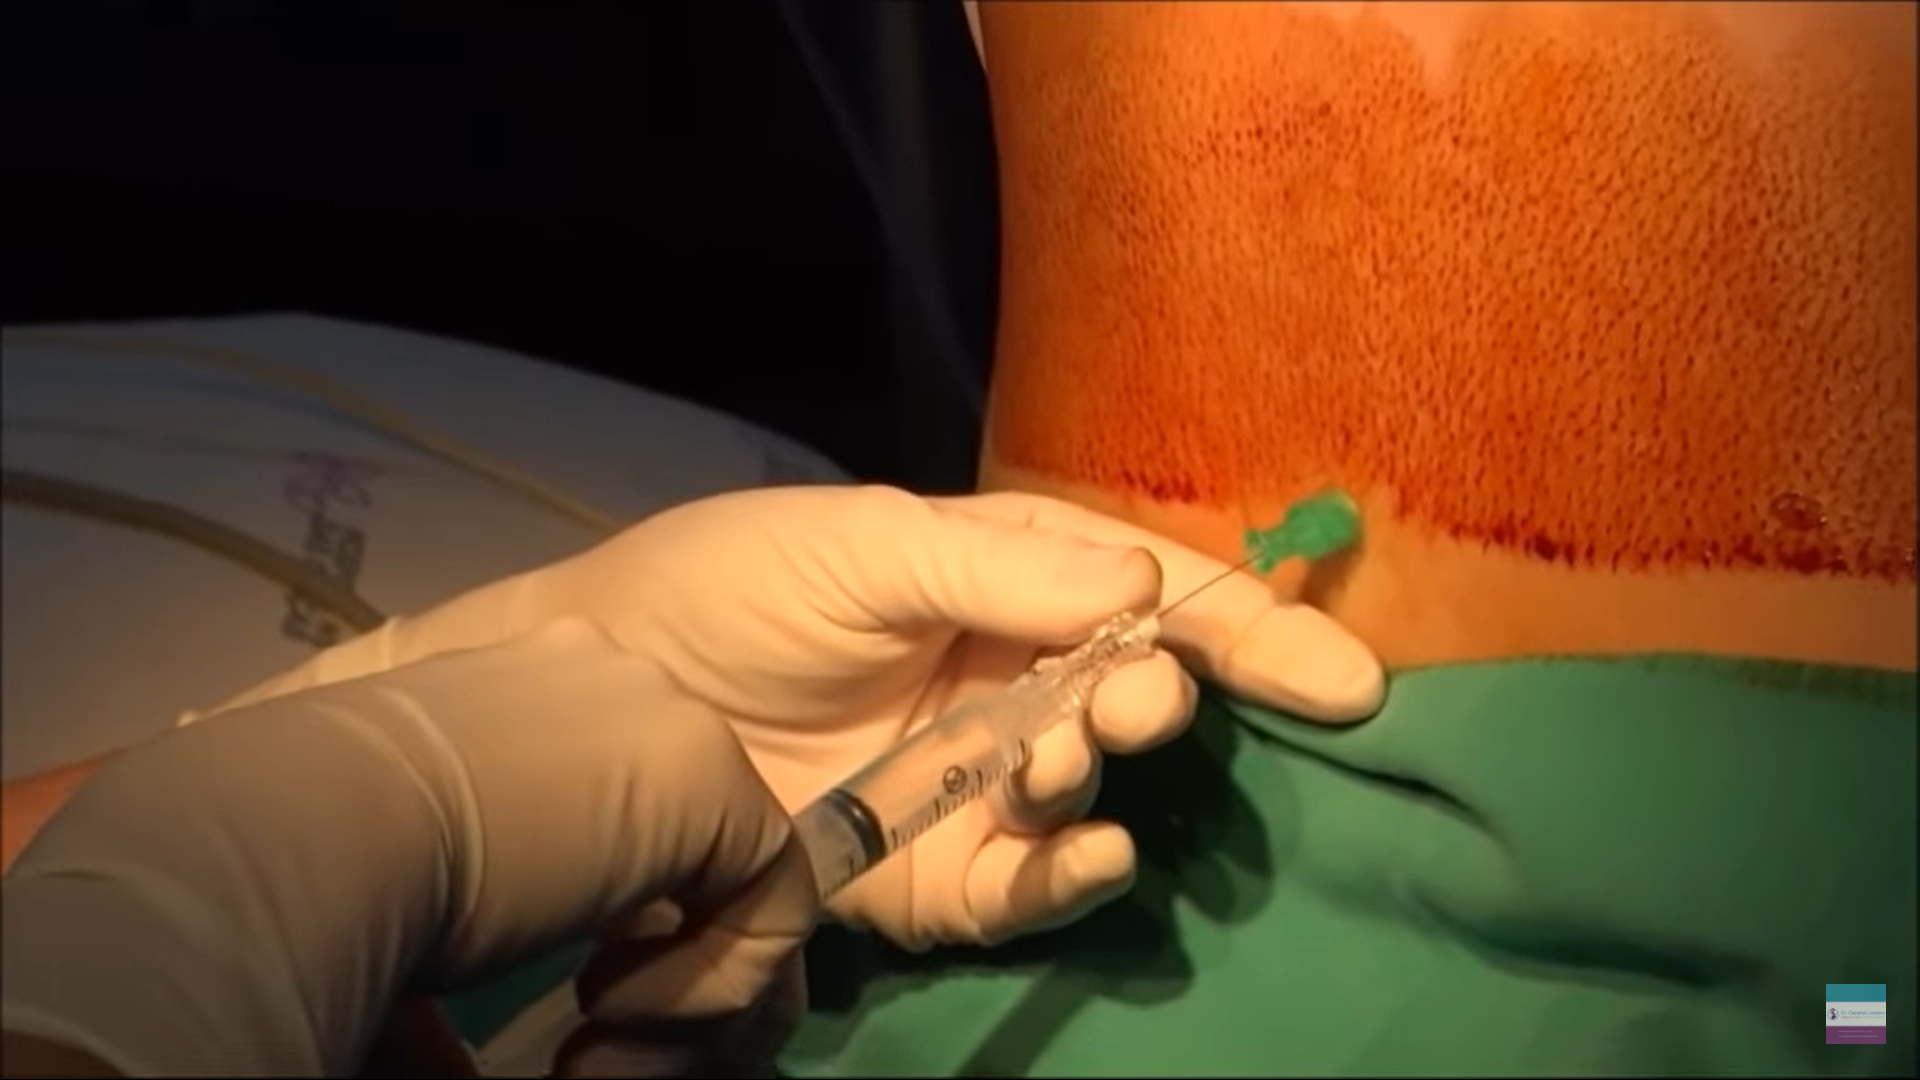
\includegraphics[width=0.6\linewidth]{capitulos/figuras/4.InjecaoAnestesico.png}
    \caption{Injeção do liquido anestésico no espaço subaracnóideo  \cite{Londero2018}.}
    \label{fig:injecaoAnestesico}
\end{figure}

Após a finalização dos procedimentos de preparação é escolhida a área onde será feita a punção através do toque da mão do médico (exemplo retirado de video na Figura~\ref{fig:marcacaoPonto}) na crista ilíaca do paciente \cite{Helayel2010,Isaacs2015}. Uma vez escolhido este ponto é feita a injeção de anestésico local (Figura~\ref{fig:anestesiaLocal}) para reduzir o desconforto na área próxima à punção \cite{Sedicias2018} Após a anestesia local é feita a inserção da agulha de punção tanto no caso da peridural como na raqui.

Existem duas principais abordagens de inserção da agulha para efetuação das anestesias regionais. Estão são denominadas mediana (do inglês \textit{midline}) e paramediana (do inglês \textit{paramedian}). A abordagem mediana é utilizada com mais frequência (96\%) \cite{Wantman2006}. Um dos motivos para o maior uso da abordagem mediana é a ausência de vasos sanguíneos no caminho da agulha nesta abordagem \cite{Bapat2015}. A abordagem paramediana é mais recomendada para pacientes idosos \cite{Ahsan-ul-Haq2005} por motivos de modificação degenerativa da coluna vertebral \cite{Boon2003} e calcificação dos ligamentos interespinhoso e supraespinhoso \cite{Wantman2006}. A abordagem paramediana também pode ser mais viável que a mediana em pacientes obesos pela dificuldade na identificação da crista ilíaca nestes pacientes. Isto por que a camada de gordura faz com que a linha média seja mais difícil de localizar através do toque do médico \cite{N.2013}. Na abordagem mediana a agulha é inserida na linha média da coluna vertebral. Na paramediana existe certa angulação entre a linha da coluna e a inserção da agulha. As duas abordagens podem ser observadas no corte transversal da coluna na Figura~\ref{fig:abordagensInsercaoAgulha}. 

\begin{figure}[ht!]
    \centering
    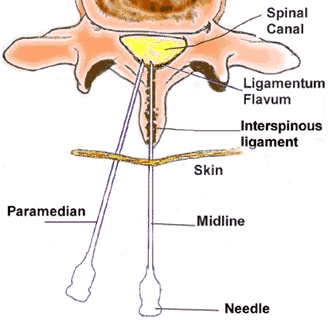
\includegraphics[width=0.6\linewidth]{capitulos/figuras/paramedian-midline-MedBroadcast-Tiff.png}
    \caption{Ilustração da abordagem mediana e paramediana para inserção de agulha \cite{MedBroadcast2018}.}
    \label{fig:abordagensInsercaoAgulha}
\end{figure}

\subsection{Anestesia Raquidiana}

Neste tipo de anestesia, uma agulha de pequeno calibre é inserida nas costas do paciente até atingir o espaço subaracnóideo (localizado após a dura-máter), dentro da coluna espinhal. Em seguida, um anestésico é injetado dentro do líquido cérebro espinhal (\textit{líquor}), produzindo dormência temporária e relaxamento muscular (Figura~\ref{fig:injecaoAnestesico}). Anestesias raquidianas são aplicadas de forma mais frequente em espaços intervertebrais abaixo da segunda vértebra lombar (L2), normalmente entre a L3 e L4 \cite{Wikipedia2019, Londero2018}. A Figura~\ref{fig:camadasPuncaoLombar} ilustra em um corte sagital da coluna as diferentes camadas que são cruzadas por uma agulha durante o procedimento de punção lombar até chegar ao espaço subaracnóideo. Considerando as duas abordagens de inserção da agulha (mediana e paramediana) as camadas onde a agulha pode passar desde a pele até o espaço subaracnóideo são: gordura subcutânea, músculo, ligamento supraespinhoso, ligamento interespinhoso, ligamento amarelo (\textit{flavum}), espaço epidural e dura-máter. O processo espinhoso que também aparece entre a pele e o espaço subaracnóideo na Figura~\ref{fig:camadasPuncaoLombar} não foi listado, pois, por ser uma camada de osso, ela não é perfurada pela agulha e sim uma camada intransponível em relação ao processo de punção.

\begin{figure}[ht!]
    \centering
    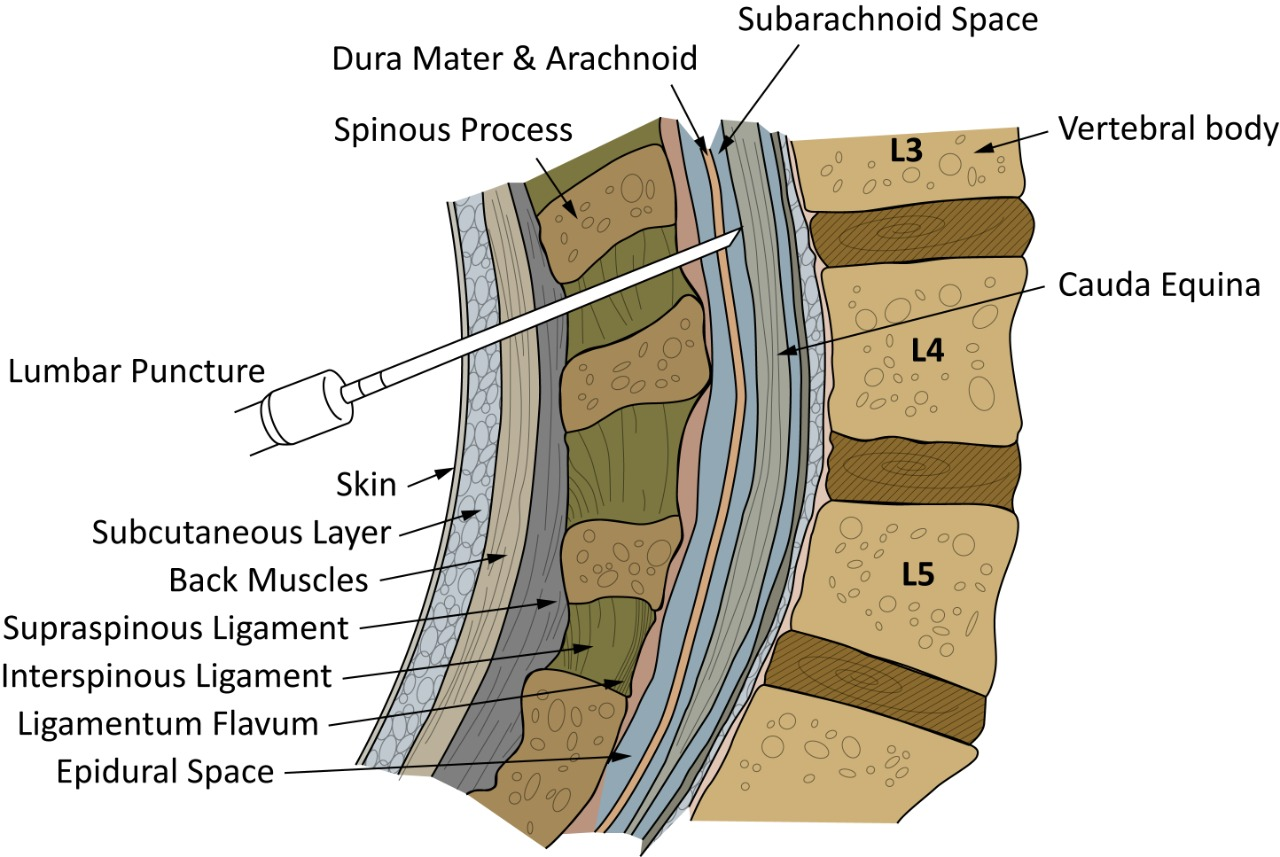
\includegraphics[width=0.6\linewidth]{capitulos/figuras/lumbar.puncture.tisssues.jpeg}
    \caption{Camadas cruzadas pela agulha numa punção lombar.}
    \label{fig:camadasPuncaoLombar}
\end{figure}

A ação do anestésico dentro da coluna espinhal é a de bloquear os nervos que passam pela coluna lombar, fazendo com que os estímulos dolorosos vindos de membros inferiores e do abdômen não cheguem ao cérebro. A raquianestesia é muito usada para procedimentos ortopédicos de membros inferiores assim como na região abdominal e cirurgias obstétricas de parto normal e cesarianas \cite{Pinheiro2018}.

A grande vantagem da anestesia raquidiana em relação a peridural é que nesta é necessário o uso de uma pequena quantidade de anestésico local. Esta característica reduz consideravelmente o risco de intoxicação por meio do elemento anestésico. Por outro lado a maior desvantagem no uso deste tipo de anestesia está na dor de cabeça que os pacientes sentem após a perfuração da dura-máter. Este sintoma é causado pela lesão na dura-máter que pode permanecer aberta por alguns dias após o procedimento, provocando perda do \textit{líquor} do espaço subaracnóideo. Com o uso de agulhas de menor diâmetro a incidência desta dor de cabeça foi consideravelmente reduzida \cite{INFOESCOLA2018}. 

\section{Realidade Virtual}

A \acrlong{RV} está presente quando se usa a tecnologia para criar a ilusão de que se está em um ambiente que não está lá ou não existe. Ela é uma aproximação da realidade experimentada por nós através dos nossos sentidos e sistemas de percepção. A nossa percepção da realidade vem através dos nossos sentidos. Portanto, uma vez apresentando aos sentidos às informações esperadas, sendo estas reais ou não, a nossa percepção da realidade irá se guiar por estes estímulos. Os sentidos mais comuns são visão, olfato, paladar, audição e tato. Porém também possuímos outros sentidos que afetam as nossas percepções do mundo, como por exemplo: o senso de equilíbrio, o sentimento de forças, pesos e deslocamentos sentidos por nossos membros \cite{VRS2018}.

Atualmente, a chamada \acrfull{RV} utiliza um computador para criar um ambiente virtual tridimensional. A intenção é a de simular uma realidade apresentando os elementos desejáveis para os sentidos do usuário, visando cumprir um objetivo através da interação de um ou mais usuários com este ambiente. Estes usuários se tornam parte deste ambiente virtual, total ou parcialmente, podendo manipular objetos ou executar um conjunto de ações \cite{VRS2018}.

A \acrshort{RV} possui uma série de usos sociais como, por exemplo, o tratamento de fobias. Há trabalhos para aracnofobia \cite{Carlin1997}, para aicmofobia ou medo de agulhas \cite{Galoustian2018}, para aerofobia ou medo de voar \cite{Rothbaum2006}, para acrofobia ou medo de altura \cite{Edwards2018} ou de forma mais geral para o medo e a ansiedade \cite{Goldman2017}. A Figura~\ref{fig:medoAltura} ilustra a aplicação para tratamento da acrofobia. Em primeiro plano a usuária com os óculos de realidade virtual e no segundo plano o ambiente virtual simulando ambientes de escadas e plataformas com fundo transparente.

\begin{figure}[ht!]
    \centering
    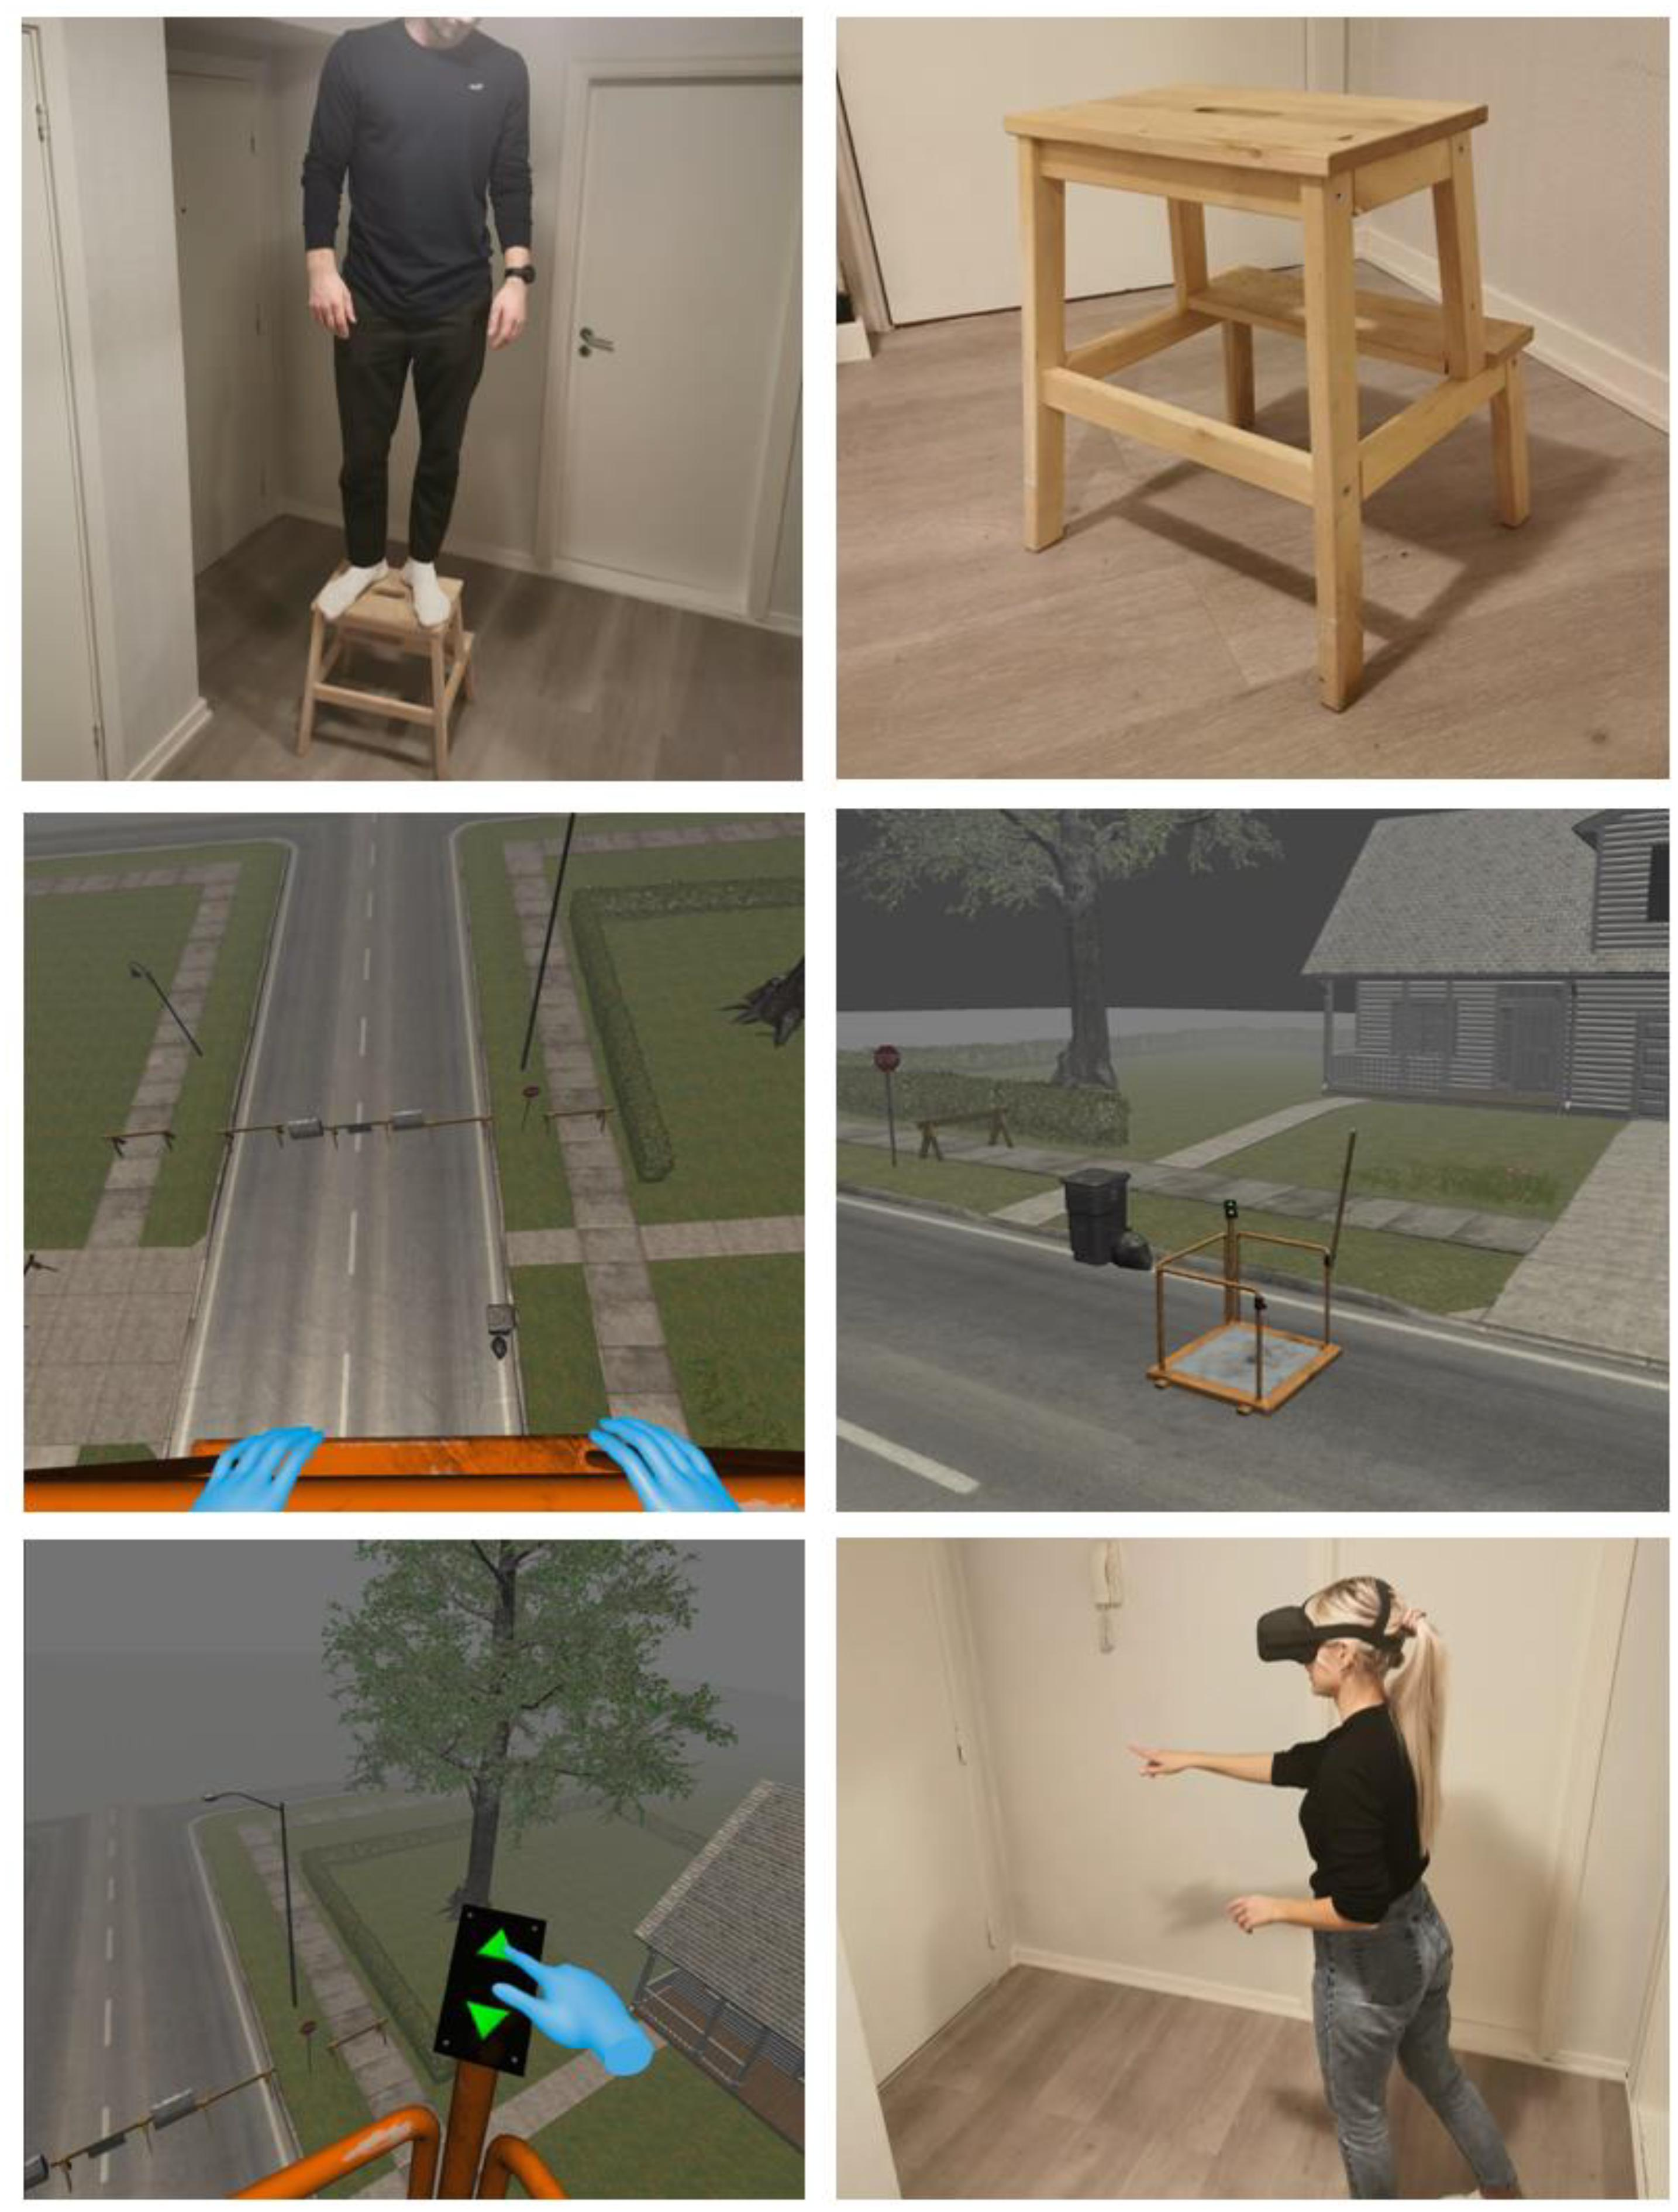
\includegraphics[width=0.6\linewidth]{capitulos/figuras/fear_of_heights.jpg}
    \caption{Exemplo de aplicação que usa \acrshort{RV} no tratamento da acrofobia \cite{Edwards2018}.}
    \label{fig:medoAltura}
\end{figure}

A indústria do entretenimento através de filmes e jogos provocou uma grande evolução de técnicas de \acrshort{RV} que posteriormente foram aplicadas em áreas mais “sérias” como o desenvolvimento pessoal e treinamento \cite{Ma2011, Prensky2001, Smith2011}. Na prática a \acrshort{RV} deve ser considerada como uma possibilidade sempre que o que se deseja fazer é muito perigoso, caro ou impraticável de ser realizado concretamente. Por conta destas características ela é muito usada nas áreas da educação, da saúde e militar \cite{VRS2018}. Conforme a tecnologia que permite a criação e simulação de ambientes virtuais se torna mais barata, mais aplicações são criadas com o uso destas ferramentas.

\section{Dispositivos Hápticos}

O termo \textit{haptics} é usado para descrever a ciência que estuda e simula a pressão, textura, vibração e outras sensações biológicas relacionadas ao toque. A sensação do toque se origina em estímulos mecânicos, elétricos, térmicos ou químicos na pele \cite{Burdea1996}. O tato não está localizado numa região específica do corpo como os demais sentidos. Ele está distribuído por todo o corpo através do órgão sensorial do toque, nossa pele, articulações, músculos e tendões. O senso do toque se divide em duas sensações: cinética e tátil. Forças e torques são sensações cinéticas que sentimos nos músculos, tendões e articulações. Já as sensações táteis como pressão, deformação e vibração são sentidas por mecano receptores que possuímos na nossa pele \cite{Culbertson2018}. 

Os primeiros dispositivos hápticos foram originados dos braços robóticos usados para o controle remoto de robôs \cite{Zurawski2005} As aplicações de tecnologias hápticas são muito variadas envolvendo, por exemplo, projetos de engenharia e aplicações de manufatura \cite{Sharma2001}, entretenimento (videogames e filmes), celulares, relógios inteligentes e até mesmo a indústria automobilística \cite{Smith2019}. Estes dispositivos possuem elementos mecânicos de entrada e saída para interação com o usuário. Uma ou mais partes do dispositivo em contato com o usuário são monitorados no espaço físico e o dispositivo oferece como retorno força e torque. Desta forma um canal bidirecional de interação entre o ambiente virtual e o usuário é criado \cite{Coles2011}. Estes dispositivos estão sendo cada vez mais utilizados hoje em dia tanto pela evolução da sua tecnologia como pela diminuição dos preços. Com o avanço da tecnologia estes dispositivos estão se tornando cada vez mais flexíveis representando mais fielmente os movimentos. Isto ocorre  através do uso de conceitos de restrição parcial a movimentos, deslocamentos e da inclusão de mais graus de liberdade, \textit{\acrfull{DoF}}. 

O número de graus de liberdade de um dispositivo háptico se refere ao número de maneiras diferentes em que este pode se mover ou criar forças. Como exemplo, dispositivos com 3 graus de liberdade podem rastrear posições e criar forças ao serem movidos nas direções: direita-esquerda, frente-trás e cima-baixo \cite{HAPTICSHOUSE2019}. O principal objetivo no uso destes dispositivos é o aumento da sensação de imersão em um ambiente de realidade virtual. 

Em relação à área médica, os dispositivos hápticos vem sendo utilizados na maioria dos trabalhos de simulação de procedimentos médicos \cite{Coles2011,Escobar-Castillejos2016}. Eles são usados para simular o uso de ferramentas em cirurgias e ajudaram a impulsionar o sucesso das práticas em simuladores virtuais. Isto aconteceu ao proporcionar o controle dos graus de liberdade de deslocamentos, a restrição aos movimentos e as respostas às atitudes do usuário como forças de reação ou \textit{feedback} \cite{Gerovich2004}. Estes dispositivos eletromecânicos existem nas mais diversas formas e são adaptados para uma grande variedade de procedimentos médicos como, por exemplo, no treinamento de laparoscopia \cite{Srinivasan2004}, biopsia de próstata \cite{Sclaverano2009}, cirurgia de fígado \cite{Mastmeyer2016}, exames de mama \cite{Brazil2017,Jeon2010,Ribeiro2014,Solanki2010}, simulação de apalpação \cite{Ribeiro2016} e punções epidurais \cite{N.2013, Brazil2018}. Alguns sistemas usam mais de um háptico como em punções de agulha guiadas por ultrassom que usam um equipamento para simular a agulha e outro para o ultrassom \cite{Ni2011,Vidal2008}. Outros chegam a fazer o uso de três dispositivos como o PalpSim de forma a simular o toque das mãos do usuário num paciente virtual \cite{Coles2011b}. 

Culbertson et al. identificaram como 3 as principais categorias de sistemas hápticos: compreensíveis, vestíveis e palpáveis. Um exemplo visual destes tipos pode ser visto na Figura 6. Os sistemas compreensíveis são dispositivos tipicamente cinéticos (\textit{feedback} de força) que normalmente possuem uma base fixa e permitem ao usuário empurrar e ser empurrado de volta. Sistemas vestíveis são tipicamente táteis montados nas mãos ou em outras partes do corpo e provocam sensações diretamente na pele. Os sistemas palpáveis são dispositivos de encontro que permitem ao usuário explorar toda a superfície \cite{Culbertson2018}. Os dispositivos a serem explorados aqui são os de sistemas compreensíveis. Estes foram os tipos de hápticos utilizados nos simuladores computacionais relacionados ao tema desta tese (seção 0) assim com nos diversos outros simuladores médicos estudados e citados nesta seção. Ribeiro et al. fizeram uma revisão sobre dispositivos usados na simulação de procedimentos que envolvem o toque da mão do médico para identificação de características e anormalidades sob a pele \cite{Ribeiro2016}. Os autores analisaram 57 trabalhos e mais da metade fez uso dos dispositivos da família \textit{Phantom}. Os dispositivos desta família serão listados na seção ===== 3 ======.

===== FIGURA ====

Nas figuras Figura 7, Figura 8, Figura 9 e Figura 10 os dispositivos aparecem representados ordenados pelas suas complexidades i.e. dos mais simples (mais antigos e com menos recursos) aos mais avançados (mais novos). Todos estes dispositivos são exemplos de sistemas tipicamente cinéticos. Os mais novos possibilitam maior número de graus de liberdade para os movimentos assim como possibilitam mais forças e momentos de reação. O Novint Falcon ® (Figura 7), lançado em 2007, tem como interface com o usuário uma esfera onde o usuário deve colocar os dedos da mão para fazer os movimentos no caso do seu uso mais comum. No que diz respeito à liberdade de movimento este mecanismo proporciona uma interação 3D com o computador no lugar da interação 2D proporcionada pelo mouse. Ele possui 3 graus de liberdade de movimento e de forças. Nesta esfera existem quatro botões para interação e existem sensores para determinar a posição do cursor e motores para controlar as forças a serem transmitidas para o usuário. Existem versões onde a esfera é substituída, por exemplo, por um dispositivo semelhante a uma pistola para que o dispositivo seja usado em jogos de tiros de primeira pessoa \cite{VRS2017}. 

===== FIGURA ====

Os hápticos da família \textit{Phantom Geomagic Touch} ® (Figura 8) e \textit{Geomagic Touch} X ® (Figura 9) apresentam uma peça que simula uma caneta para manipulação do usuário da mesma forma que a esfera no dispositivo da Figura 7. Nas canetas também existem botões para interação e da mesma forma estas também são substituíveis por partes com formas mais adequadas ao procedimento que estas pretendem simular. O dispositivo \textit{Geomagic Touch} X ® possui a mesma liberdade de movimento do \textit{Geomagic Touch} ®, porém possibilita \textit{feedback} de reações maiores. Ambos apresentam 6 graus de liberdade de movimento e 3 graus de liberdade no retorno de forças. Estes dispositivos, portanto mapeiam a posição 3D e orientação, mas somente apresentam \textit{feedback} de forças direcionais \cite{Forsslund2013}.

===== FIGURA ====

===== FIGURA ====

O \textit{Phantom Premium} ® (Figura 10) está disponível nas versões \textit{Premium} 1.0, \textit{Premium 1.5} e 1.5/HF, e \textit{Premium} 3.0. Estas evoluem não só o \textit{feedback} de reações como também os graus de liberdade dos movimentos. Enquanto o \textit{Phantom Premium} 1.0 ® simula o movimento do giro do pulso na mão o \textit{Phantom Premium} 3.0 ® possibilita uma amplitude que simula os graus de liberdade de movimento de todo o braço humano desde o ombro \cite{3DSystems2018}. Este dispositivo possui 6 graus de liberdade tanto para movimento como retorno de forças o que o torna simétrico no número de sensores e motores (atuadores). São computadas forças e torques tanto da posição como da orientação deste dispositivo. Esta característica tem uma forte influencia no alto custo associado a este tipo de dispositivo \cite{Forsslund2013}.

===== FIGURA ====

=========

\section{Modelagem de tecidos}

Um dos passos necessários para construção de um ambiente virtual para treinamento de anestesia epidural e raquianestesia é a criação de pacientes virtuais. Um importante aspecto da modelagem destes pacientes é como eles aparecem na tela da aplicação. Outro aspecto importante na simulação é ter uma estimativa da espessura dos tecidos envolvidos nestes tipos de anestesia. Para isto é necessária à modelagem do tamanho de todas as camadas de tecido pelos quais as agulhas passam para execução destes procedimentos. Uma ilustração destes tecidos que vão desde a pele até a dura-máter pode ser vista na Figura 3. Nesta seção são descritos trabalhos relacionados com a modelagem da distância entre a pele e a dura-máter.

Na Tabela 2 são listadas as varáveis de entrada e saída dos métodos estudados nesta seção. Esta tabela exibe também as unidades destas variáveis que serão utilizadas em todo este trabalho.

===== TABELA ====

Muitos trabalhos buscam relacionar a distância que vai da superfície externa da pele até o espaço epidural (DEE) com as demais variáveis da Tabela 2. A grande maioria dos trabalhos indica uma forte relação da DEE com o IMC \cite{Adegboye2017, Galbraith2018}. Estes dois trabalhos não fazem separação dos grupos populacionais por idade, sexo ou etnia, e usaram populações respectivamente de n=120 e n=317 pessoas entre homens e mulheres.

Os trabalhos citados a seguir analisaram somente ou de forma separada grupos de mulheres grávidas. Como este é o foco deste trabalho só serão comentadas aqui as conclusões referentes a estes grupos. Todos os trabalhos a seguir encontraram influencia do IMC na determinação da DEE, mas além desta relação também foram encontradas outras combinações em cada trabalho. O grupo étnico/populacional do individuo foi observado em conjunto com o IMC em \cite{Sharma2011} estudo feito no Reino Unido. A idade foi observada em conjunto com o IMC num estudo em pacientes americanas em Michigan, EUA \cite{Clinkscales2007}. A altura, massa, idade e IMC foram observados como relevantes em um estudo em pacientes da Índia \cite{Hazarika2016}. Estes dois últimos trabalhos construíram equações de regressão linear para determinação da DEE para grupos de parturientes conforme pode ser visto na Tabela 3.

===== TABELA ====

Os autores em \cite{Sharma2011} no lugar das equações apresentaram como resultado uma tabela com cinco pontos de cada par IMC x DEE para cada grupo populacional analisado. Estes dados podem ser vistos na Tabela 4. A definição dos grupos populacionais no estudo do Reino Unido (RU) em \cite{Sharma2011} foi: Brancas (população do Reino Unido, da Irlanda e qualquer outro grupo com cor de pele branca); Asiáticas ou Britânicas Asiáticas (população da Índia, Paquistão, Bangladesh ou qualquer outro grupo Asiático); Negras ou Britânicas negras (população de Africanas, Caribenhas ou outros grupos com cor da pele negra); e Chinesas e outros grupos étnicos (população da China, Japão, Malásia, Filipinas etc.). No grupo de nome Chinesas, além dos dados de pessoas desta origem moradoras do Reino Unido, foram considerados dados de Chinesas (n=70) de um hospital de Singapura.

===== TABELA ====

Na Tabela 5 é apresentado o tamanho da população utilizada nestes estudos e as identificações da origem dos dados do estudo, isto é, os grupos populacionais analisados. 

===== TABELA ====

A listagem dos tecidos entre a pele e a DEE e a relação dessa distância com o aumento de peso é comentada em \cite{Palmer1983}. Os autores concluem que com o aumento do peso/massa (do paciente) o tecido que sofre a maior variação é a gordura subcutânea.

Na seção = ==== é proposto o uso de dados de trabalhos comentados aqui para modelagem de tecidos de pacientes grávidas.

=========

Este capítulo apresentou uma fundamentação teórica sobre ====. Iniciou apresentando ==========. Logo em seguida o capítulo apresenta ====== e suas principais entidades e que estão relacionadas com a proposta desta tese. O capitulo finaliza apresentando os conceitos que envolvem ==== e seus principais elementos. O próximo capítulo oferece uma visão das pesquisas relacionadas ao tema desta tese e compara-as com as proposições que foram colocadas ao longo deste trabalho. Essas pesquisas tratam e ========== assim como de ===========.


% --- -----------------------------------------------------------------
% --- Referencias Bibliograficas. (Obrigatorio)
% --- -----------------------------------------------------------------
\cleardoublepage

 %para personalização da bibliografia olhar os PDFs na pasta "MANUAIS"
\printbibliography[
   % heading=bibintoc,
    title={REFERÊNCIAS} %TITULO DA SEÇÃO
] 

% --- -----------------------------------------------------------------
% --- Apendice.(Opcional)
% --- -----------------------------------------------------------------
\cleardoublepage
\appendix
%para melhor organização deixar os Anexos e Apêndices na pasta anexos.
\chapter{Projeto aprovado no comitê de ética via plataforma Brasil}
\label{apend}

\begin{figure}[htp] \centering{
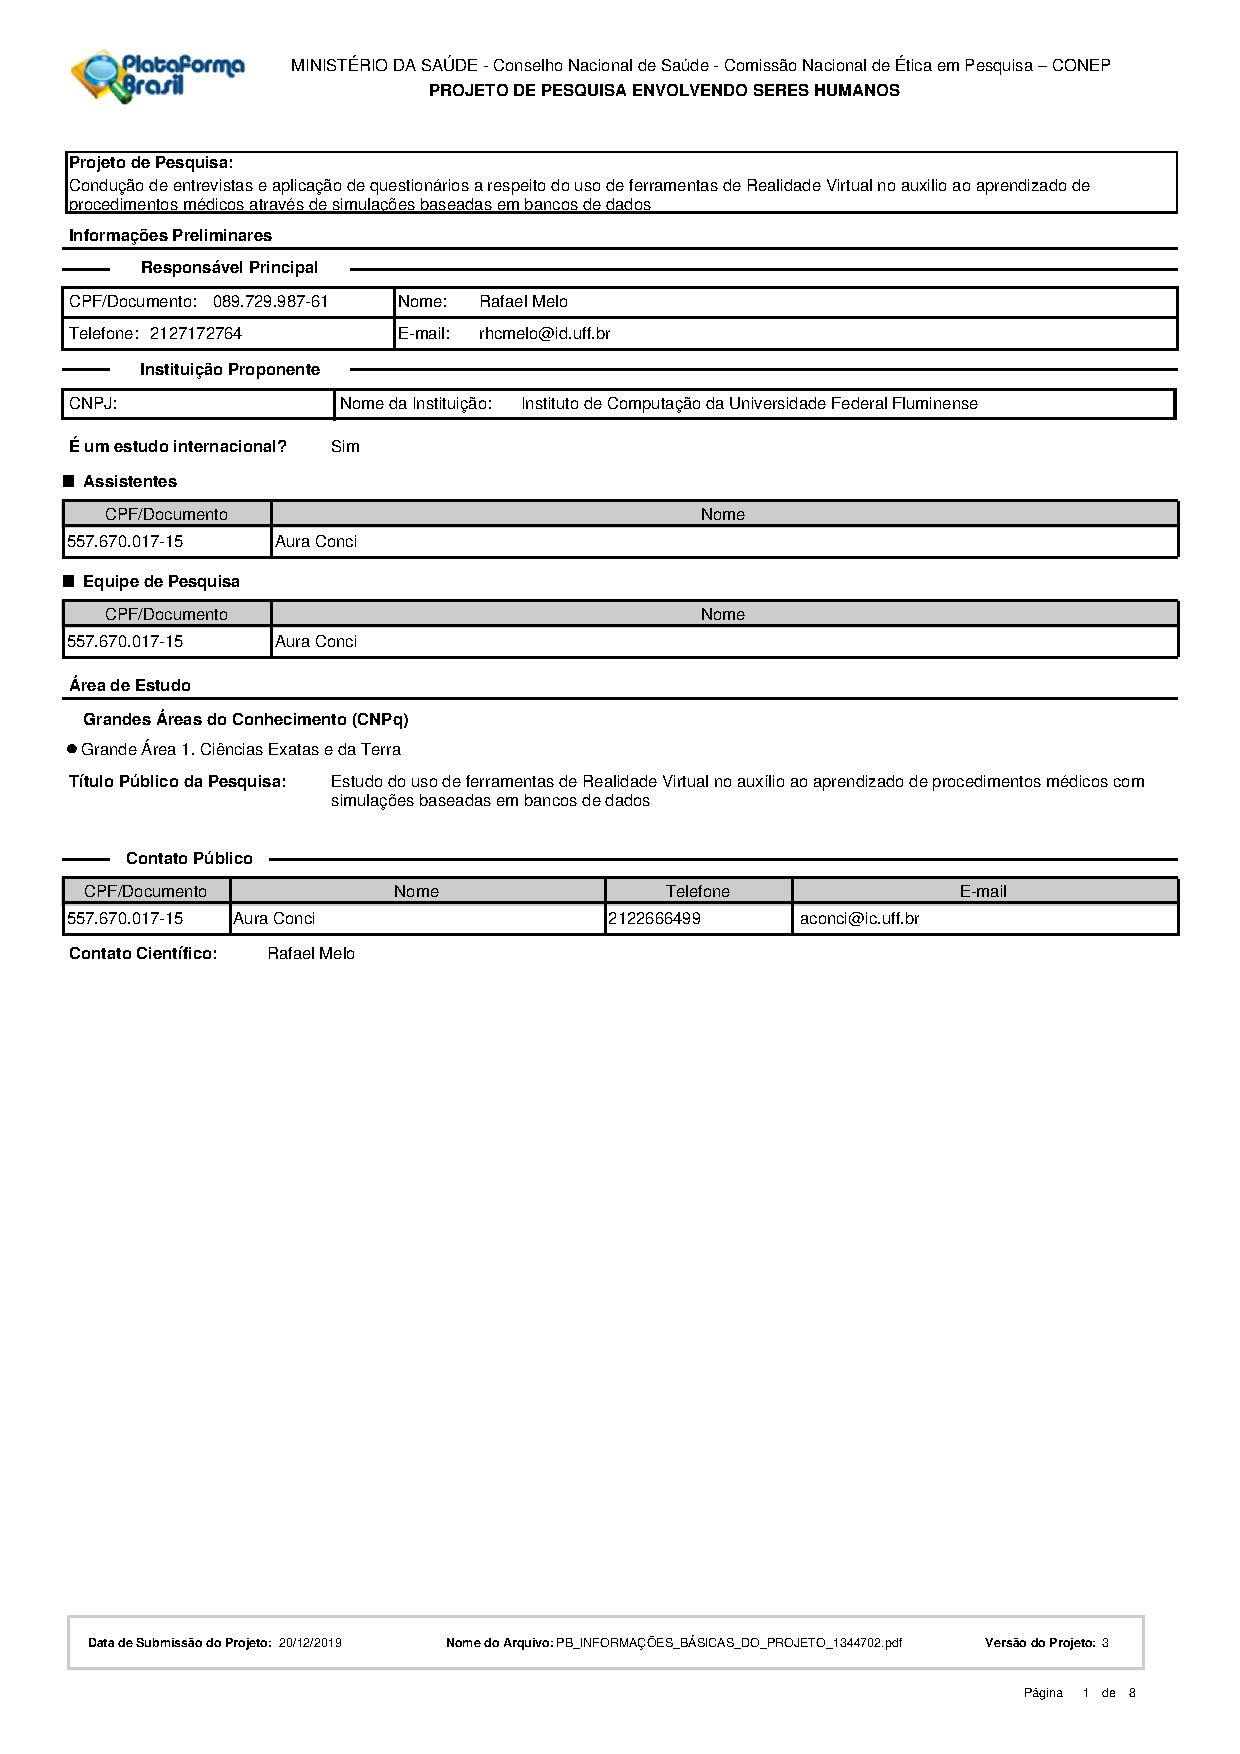
\includegraphics[scale=0.82]{pos-textuais/apendices/PB_INFORMAÇÕES_BÁSICAS_DO_PROJETO_1344702.pdf}
\caption{Experiment 1}
\end{figure}

% Este apêndice apresenta informações complementares.

%Elemento opcional. O(s) apêndice(s) são identificados por letras maiúsculas consecutivas, travessão e pelos respectivos títulos. Excepcionalmente utilizam-se letras maiúsculas dobradas, na identificação, quando esgotadas as 23 letras do alfabeto (ABNT, 2005).



\chapter{ANEXO A – TÍTULO DO ANEXO}
\label{lab:anexoA}

"Elemento opcional. O(s) anexo(s) são identificados por letras maiúsculas consecutivas, travessão e pelos respectivos títulos. Excepcionalmente utilizam-se letras maiúsculas dobradas, na identificação dos anexos, quando esgotadas as 23 letras do alfabeto" (ABNT, 2005).


\end{document}

